% arara: pdflatex: { synctex: yes }
% arara: makeindex: { style: ctuthesis }
% arara: bibtex

% The class takes all the key=value arguments that \ctusetup does,
% and a couple more: draft and oneside
\documentclass[oneside]{ctuthesis}

\usepackage{siunitx}
\usepackage{nomencl}
\usepackage{setspace}
\usepackage{indentfirst}

%%%%%%%%%%%%%%%%%% insert images from other directory
\usepackage{graphicx}
\graphicspath{{./images/}}


\usepackage{pdfpages}	
\usepackage{longtable}


%%%%%%%%%%%%%%%%%%%%%%%%%%%%%%%%%%%%%% this shit is here to break long url into more lines
\usepackage{url}
\makeatletter
\g@addto@macro{\UrlBreaks}{\UrlOrds}
%\makeatother

%%%%%%%%%%%%%%%%%%%%%%%%%%%%%%%%%%%%%% this shit is here to prevent breaking words on the edge of a line
\tolerance=1
\emergencystretch=\maxdimen
\hyphenpenalty=10000
\hbadness=10000


%%%%%%%%%%%%%%%%%%%%%%%%%%%%%%%%%%%%%% force urls in the bibliography to split
\def\UrlBreaks{\do\/\do-\do9}
\usepackage{breakurl}

 
%%%%%%%%%%%%%%%%%%%%%%%%%%.this makes the differed text make different
%DIF PREAMBLE EXTENSION ADDED BY LATEXDIFF
%DIF UNDERLINE PREAMBLE %DIF PREAMBLE
\RequirePackage[normalem]{ulem} %DIF PREAMBLE
\RequirePackage{color}\definecolor{RED}{rgb}{1,0,0}\definecolor{BLUE}{rgb}{0,0,1} %DIF PREAMBLE
\providecommand{\DIFadd}[1]{{\protect\color{blue}\uwave{#1}}} %DIF PREAMBLE
\providecommand{\DIFdel}[1]{{\protect\color{red}\sout{#1}}}                      %DIF PREAMBLE
%DIF SAFE PREAMBLE %DIF PREAMBLE
\providecommand{\DIFaddbegin}{} %DIF PREAMBLE
\providecommand{\DIFaddend}{} %DIF PREAMBLE
\providecommand{\DIFdelbegin}{} %DIF PREAMBLE
\providecommand{\DIFdelend}{} %DIF PREAMBLE
%DIF FLOATSAFE PREAMBLE %DIF PREAMBLE
\providecommand{\DIFaddFL}[1]{\DIFadd{#1}} %DIF PREAMBLE
\providecommand{\DIFdelFL}[1]{\DIFdel{#1}} %DIF PREAMBLE
\providecommand{\DIFaddbeginFL}{} %DIF PREAMBLE
\providecommand{\DIFaddendFL}{} %DIF PREAMBLE
\providecommand{\DIFdelbeginFL}{} %DIF PREAMBLE
\providecommand{\DIFdelendFL}{} %DIF PREAMBLE
%DIF END PREAMBLE EXTENSION ADDED BY LATEXDIFF


% to print code
\usepackage{listings}
\usepackage{color}
\definecolor{dkgreen}{rgb}{0,0.6,0}
\definecolor{gray}{rgb}{0.5,0.5,0.5}
\definecolor{mauve}{rgb}{0.58,0,0.82}
\lstset{frame=tb,
  language=C++,
  aboveskip=3mm,
  belowskip=3mm,
  showstringspaces=false,
  columns=flexible,
  basicstyle={\small\ttfamily},
  numbers=none, 
  % numberstyle=\tiny\color{gray},
  % keywordstyle=\color{blue},
  % commentstyle=\color{dkgreen},
  % stringstyle=\color{mauve},
  breaklines=true,
  breakatwhitespace=true,
  tabsize=3
}
% to display source code
\definecolor{mGreen}{rgb}{0,0.6,0}
\definecolor{mGray}{rgb}{0.5,0.5,0.5}
\definecolor{mPurple}{rgb}{0.58,0,0.82}
\definecolor{backgroundColour}{rgb}{0.95,0.95,0.92}
\lstdefinestyle{CStyle}{
    backgroundcolor=\color{backgroundColour},   
    commentstyle=\color{mGreen},
    keywordstyle=\color{magenta},
    numberstyle=\tiny\color{mGray},
    stringstyle=\color{mPurple},
    basicstyle=\footnotesize,
    breakatwhitespace=false,         
    breaklines=true,                 
    captionpos=b,                    
    keepspaces=true,                 
    numbers=left,                    
    numbersep=5pt,                  
    showspaces=false,                
    showstringspaces=false,
    showtabs=false,                  
    tabsize=2,
    language=C
}
\lstdefinestyle{log}{
    backgroundcolor=\color{backgroundColour},   
    % commentstyle=\color{mGreen},
    % keywordstyle=\color{magenta},
    % numberstyle=\tiny\color{mGray},
    % stringstyle=\color{mPurple},
    basicstyle=\footnotesize,
    breakatwhitespace=false,         
    breaklines=true,                 
    % captionpos=b,                    
    keepspaces=true,                 
    numbers=none,                    
    numbersep=5pt,                  
    showspaces=false,                
    showstringspaces=false,
    showtabs=false,                  
    tabsize=2,
    language=C
}


%%%
% \usepackage{framed}
% \usepackage{hyperref}
% % \usepackage[czech]{babel}
% \usepackage[utf8]{inputenc}
% \usepackage[T1]{fontenc}

\usepackage{dirtree}        %directory tree visualisation
\usepackage{blindtext}
\parskip=12pt % adds vertical space between paragraphs

\usepackage{xcolor}
\definecolor{shadecolor}{RGB}{230,230,230}

% to print code
\usepackage{listings}
\usepackage{color}
%%%

\ctusetup{
%	preprint = \ctuverlog,```%%%%%%%%%%%%%%%%%%%%%%%%% toto je cislo na kazde strance dole ktere tam nema byt
%	mainlanguage = english,
%	titlelanguage = english,
	mainlanguage = czech,
	otherlanguages = {czech},
	% title-czech = {Low power wireless sensor network},
	title-czech = {Bezdrátová senzorová síť pro přístupový systém},
	title-english = {Wireless sensor network for access control system},
	subtitle-czech = {},
	subtitle-english = {},
	faculty = F3,
	department-czech = {Katedra telekomunikační techniky},
	department-english = {Department of Telecommunications Engineering},
	author = {Bc. Tomáš Hyhlík},
	supervisor = {Ing. Bc. Marek Neruda, Ph.D},
	supervisor-address = {},
	supervisor-specialist = {doc. Ing. Lukáš Vojtěch, Ph.D},
	fieldofstudy-english = {Electronics and Communications},
	subfieldofstudy-english = {Electronics},
	fieldofstudy-czech = {Elektronika a komunikace},
	subfieldofstudy-czech = {Elektronika},
	keywords-czech = {LoRa, LPWAN, přístupový systém, WSN.},
	keywords-english = {Access control system, LoRa, LPWAN, WSN.},
	day = 20,
	month = 5,
	year = 2020,
	specification-file = {zav_prace.pdf},
%	front-specification = true,
%	front-list-of-figures = false,
%	front-list-of-tables = false,
%	monochrome = true,
%	layout-short = true,
}

\ctuprocess

\addto\ctucaptionsczech{%
	\def\supervisorname{Vedoucí}%
	\def\subfieldofstudyname{Studijní program}%
}

\ctutemplateset{maketitle twocolumn default}{
	\begin{twocolumnfrontmatterpage}
		% \ctutemplate{twocolumn.thanks}
		% \ctutemplate{twocolumn.declaration}
		\ctutemplate{twocolumn.abstract.in.titlelanguage}
		\ctutemplate{twocolumn.abstract.in.secondlanguage}	
		\ctutemplate{twocolumn.tableofcontents}
		\ctutemplate{twocolumn.listoffigures}
	\end{twocolumnfrontmatterpage}
}

% Theorem declarations, this is the reasonable default, anybody can do what they wish.
% If you prefer theorems in italics rather than slanted, use \theoremstyle{plainit}
\theoremstyle{plain}
\newtheorem{theorem}{Theorem}[chapter]
\newtheorem{corollary}[theorem]{Corollary}
\newtheorem{lemma}[theorem]{Lemma}
\newtheorem{proposition}[theorem]{Proposition}

\theoremstyle{definition}
\newtheorem{definition}[theorem]{Definition}
\newtheorem{example}[theorem]{Example}
\newtheorem{conjecture}[theorem]{Conjecture}

\theoremstyle{note}
\newtheorem*{remark*}{Remark}
\newtheorem{remark}[theorem]{Remark}

\setlength{\parskip}{5ex plus 0.2ex minus 0.2ex}

% Abstract in Czech
\begin{abstract-czech}
Senzorové sítě hrají důležitou roli v internetu věcí (IoT). Jsou vhodné pro aplikace v budovách, umožňující pohodlně sbírat data ze senzorů a ovládání aktuátorů v budově a jejím okolí.  
	%Nowadays, existing intelligent buildings include some electronic systems, such as access control systems. 
	%As the WSN becomes neccesary, the effort of imlementation of WSN into existing smart buildings grow.
	%It may be easier and cheaper to extend an existing electronic system with WSN instead of integrating an entire new WSN system into the building.
Tato práce obsahuje návrh rozšíření existujícího přístupového systému o senzorovou síť. 
Je zde navržena jednokanálová LoRa gateway senzorové sítě připojena do sítě RS485 přístupového systému. 
Výsledky měření dlouhodobého provozu v jednom bloku univerzity ukazují, že maximální počet koncových zařízení senzorové sítě současně odesílajících data na gateway, může být až stovky či tisíce v závislosti na použité přenosové rychlosti dat sítě RS485 přístupového systému a použité rezervě přenosové rychlosti dat, která zabraňuje selhání funkce přístupového systému. Výsledky dokazují, že navrženou senzorovou síť lze efektivně využít v této infrastruktuře.
Dále jsou zde diskutovány možnosti vylepšení navrženého řešení a je proveden návrh vylepšení prototypu navržené gatewaye.
\end{abstract-czech}

% Abstract in English
\begin{abstract-english}
The Wireless Sensor Network (WSN) plays an important role in the Internet of Things (IoT). 
It is very suitable for intelligent buildings providing a convenient way to collect sensor data and control electronic devices in the building and its surroundings.
%Nowadays, existing intelligent buildings include some electronic systems, such as access control systems. 
%As the WSN becomes neccesary, the effort of imlementation of WSN into existing smart buildings grow.
%It may be easier and cheaper to extend an existing electronic system with WSN instead of integrating an entire new WSN system into the building.
This work proposes an extension of the existing access control system with WSN. Design of single-channel LoRa gateway connected to the existing RS485 network is performed. The results of a long-term operation measurement in one university floor show the maximum number of sensor nodes simultaneously transmitting data in RS485 network is up to hundreds or thousands in dependence on used RS485 data rate and used reserve of data rate which prevent from malfunction of the access control system. The results prove the WSN can be effectively used in an existing RS485 infrastructure. 
There are also discussed conditions of improvement of the design and upgrade of the designed gateway is performed.
\end{abstract-english}


% Acknowledgements / Podekovani
\begin{thanks}
Rád bych poděkoval lidem, kteří se na této práci podíleli, to jsou z univerzity ČVUT FEL Ing. Bc. Marek Neruda Ph.D, Ing. Bc. Pavel Bezpalec Ph.D a doc. Ing. Lukáš Vojtěch Ph.D a z firmy IMA Ing. Vlastimil Beneš. 
% za poskytnutí informací, prostředků a pomoci v rámci práce s přístupovým systémem.
\end{thanks}


% Declaration / Prohlaseni
\begin{declaration}
Prohlašuji,  že  jsem  předloženou  práci  vypracoval samostatně a že jsem uvedl veškeré použité informační zdroje v souladu s Metodickým pokynem o dodržování etických principů při přípravě vysokoškolských závěrečných prací.

V Praze, \ctufield{day}.~\monthinlanguage{title}~\ctufield{year}

% I declare that I have developed the presented work independently and that I have
% listed all information sources used in accordance with the Methodical Guidelines on
% Maintaining Ethical Principles During the Preparation of Higher Education Theses.

% In Prague, \ctufield{day}.~\monthinlanguage{title}~\ctufield{year}
\end{declaration}

% Only for testing purposes
\listfiles
\usepackage[pagewise]{lineno}
\usepackage{lipsum,blindtext}
\usepackage{mathrsfs} % provides \mathscr used in the ridiculous examples

\newcommand{\abbrlabel}[1]{\makebox[3cm][l]{\textbf{#1}\ \dotfill}}
\newenvironment{abbreviations}{\begin{list}{}{\renewcommand{\makelabel}{\abbrlabel}}}{\end{list}}


%%%%%%%%%%%%%%%%%%%%%%%%%%%%%%%%%  BEGIN %%%%%%%%%%%%%%%%%%%%%%%%%%%%%%%%%%%%%%%%%
\begin{document}



\maketitle

\includepdf[pages={1}]{zav_prace.pdf}


% \ctutemplate{specification.as.chapter}       % ZADANI

%\rule{\linewidth}{1pt}     % this shit was here for the url cut
\titlespacing*{\chapter}					{0pt}	{0ex}{0ex}
\titlespacing*{\section} 					{0pt}	{0ex}{-3ex}
\titlespacing*{\subsection} 			{0pt}	{0ex}{-3ex}
\titlespacing*{\subsubsection}		 {0pt}	{0ex}{-4ex}
\titlespacing*{\paragraph} 			{0pt}	{0ex}{-4ex}
\titlespacing*{\aubparagraph} 		{0pt}	{0ex}{-4ex}


% \setcounter{secnumdepth}{0} %% no section numbering

% \section{List of Abbreviations}
\section{Seznam zkratek}
\begin{abbreviations}
	\item[AES]		Advanced Encryption Standard 
	\item[AI]		Artifical Inteligence
	\item[AppSKey]	Application Session Key	
	\item[ASCII] 	American Standard Code for Information Interchange
	\item[BLE]		Bluetooth Low Energy 
	\item[CMAC]		Cipher-based message authentication code 
	\item[CMSIS]	Cortex Microcontroller Software Interface Standard  
	\item[CPU]		Central Processing Unit
	\item[CR] 		Carriage Return
	\item[CRC] 		Cyclic Redundancy Check
	\item[EEPROM] 	Electrically Erasable Programmable Read-Only Memory
	\item[FIFO]		First In First Out 
	\item[GPIO]		General Purpose Input Output 
	\item[HAL]		Hardware Abstraction Layer 
	\item[HW]		HardWare
	\item[IDE]		Integrated Development Environment 
	\item[IoT] 		Internet of Things
	\item[ISM]		Industrial, scientific and medical 
	\item[IWDG]		Independent Watchdog 
	\item[LAN]		Local Area Network
	\item[LBT]		Listen Before Talk 
	\item[LF]		Line Feed 
	\item[LPWAN]   	Low Power Wide Area Network 
	\item[LPWSN] 	Low Power Wireless Sensor Network	
	\item[LTE-M] 	Long Term Evolution-Machine Type Communication 
	\item[MCU] 		Micro Controller Unit
	\item[NB-IoT] 	NarrowBand-Internet of Things   
	\item[NwkSKey]	Network Session Key
	\item[PC]		Personal Computer 
	\item[PCB]		Printed Circuit Board 
	\item[RF]		Radio Frequency
	\item[RTOS]		Real Time Operating System 
	% \item[I2C]   	Inter-integrated Circuit
	% \item[IPv6] 	Internet Protocol version 6
	% \item[M2M]		machine to machine
	% \item[RPMA]		Random Phase Multiple Access
	\item[SDK]	 	Software development kit
	\item[SF]		Spreading Factor
	\item[SPI]   	Serial Peripheral Interface 
	\item[SWP]		Single Wire 
	\item[TTN] 		The Things Network
	\item[UART]		Universal Asynchronous Receiver Transmitter 
	\item[UID]		Unique Identifier 
	\item[ULP]		Ultra Low Power 
	\item[USB]		Universal Serial Bus 
	\item[WSN]		Wireless Sensor Network

\end{abbreviations}

% \setcounter{secnumdepth}{1} %% start section numbering



%%%%%%%%%%%%%%%%%%%%%%%%%%%%%%%%%%%%%%%%%%%%%%%%
% \chapter{The purpose of low power wireless sensor networks and its state of art}
\chapter{Úvod}
Se stále rostoucím využitím IoT (Internet of Things) aplikací v různých oblastech, např. zemědělství, smart metering, smart cities, smart homes, roste i počet dostupných bezdrátových technologií se zaměřením na 
nízkou spotřebu energie, velký dosah, nízkou přenosovou rychlost a nízkou cenu.

IoT aplikace vyžadující krátký dosah, jako je použití v domácnostech (smart home) většinou využívají bezdrátové technologie Zigbee nebo Bluetooth, tedy technologie používající pásmo ISM (Industrial Scientific and Medical) 2.4 GHz \cite{Design and Implementation of an IoT Assisted Real Time ZigBee Mesh WSN}, \cite{Internet of Things (IoT) for building Smart Home System}.
IoT aplikace vyžadující dlouhý dosah jsou vetšinou založené na druhu technologií LPWAN (Low Power Wide Area Network) \cite{A comparative study of LPWAN technologies for large-scale IoTdeployment}. Mezi nejpoužívanější z této kategorie, založené na bezlicenčním pásmu ISM, jsou LoRa a SigFox, a založené na licenčním pásmu jsou NB-IoT (NarrowBand-Internet of Things) a LTE-M (Long Term Evolution-Machine Type Communication).
LPWAN technologie mají dosah 10–15 km v oblastech mimo město a 2–5 km v městských oblastech \cite{Long-Range Communications in Unlicensed Bands}. Topologie LPWAN sítí jsou hvězdice (centralizovaná), hvězdice z hvězdic (decentralizovaná) a mesh (distribuovaná) \cite{high density LPWAN}.
Nízká spotřeba koncových zařízení senzorových sítí jim umožňuje dlouhou životnost z baterie, i delší než 10 let.
Nízké ceny HW (Hardware) je dosaženo úplnou integrací transceiverů s minimálním množstvím komponentů mimo čip \cite{MURS Band for LPWAN Applications}. 


Průmysl IoT roste, protože má obrovský potenciál. Cisco studie \cite{IoT cisco study} uvádí, že IoT bude kombinováno s dalšími technologiemi, jako je umělá inteligence, fog computing a blockchain. Takovéto kombinace technologií vytvoří vyšší hodnotu investice pro firmy.
IoT aplikace v oblasti smart cities požadují škálovatelné pokrytí sítě. Toho je možné dosáhnout propojením několika gatewayí, jak je navrženo v \cite{Flexible Wireless Sensor Network for smart lighting applications}, kde všechny gatewaye jsou připojeny k web serveru přístupným přes internet a cílem tohoto sytému je řídit městské veřejné osvětlení a do budoucna je plánováno použití pro měření (smart metering).
Podobná aplikace je navržena v \cite{Design and Implementation of an IoT Assisted Real Time ZigBee Mesh WSN}, která se zaměřuje na automatické měření ve městě, ale škálovatelný dosah je zajištěn topologií sítě mesh.
IoT aplikace v konceptu budov (mart buildings) jsou běžně navrženy tak, že zařízení v síti jsou připojeny ke cloudu přes Bluetooth gateway nebo Wi-Fi router připojený k internetu \cite{Internet of Things (IoT) for building Smart Home System}.
Podobná aplikace je navržena  v \cite{Building a Smart Home System with WSN and Service Robot}, kde v Zigbee síti jsou zařízení ovládána jedním zařízením typu master, které je připojeno k PC přes RS232.
Základní systém měření (smart metering) je možné vytvořit pomocí zařízení se senzory připojených ke gatewayi senzorové sítě, která je připojena k PC, kde jsou data ze senzorů zaznamenávány a vyhodnocovány \cite{A Meter Reading System Based on WSN}, \cite{Smart Water Meter System for User-Centric Consumption Measurement}, \cite{Radio Data Infrastructure for Remote Monitoring}.
Měřící systémy vyžadující velký dosah mohou být navrženy použitím více gatewayí připojených k serveru, ze kterého jsou pak data získávána aplikačním serverem \cite{Smart Electric Meter Using LoRA Protocols and Iot applications}. 
Na tomto principu funguje např. TTN (The Things Network) \cite{ttn}, což je otevřená LoRaWAN síť, do které uživatelé zdarma připojují vlastní koncová zařízení a gatewaye. Data z koncových zařízení jsou odesílány na TTN server odkud je uživatelé získávají vlastním aplikačním serverem. Uživatel tak může využívat gatewaye TTN sítě instalované jinými uživateli. Pokud potřebuje pokrytí TTN sítě v místě, kde doposud není, může v tomto místě instalovat vlastní TTN gateway a tím rozšířit pokrytí TTN sítě pro všechny uživatele.
% Similar network is proposed in Smart Farm application \cite{Implement Smart Farm with IoT Technology} with the difference that nodes can also be connected to the gateway via RS485 which forms a hybrid wired /wireless system.


Tato práce se zabývá návrhem rozšíření přístupového systému o senzorovou síť nebo-li WSN (Wireless Sensor Network) se zameřením na nízkou spotřebu energie, která by mohla být využita pro aplikace smart metering, smart buildings a v okolí budovy aplikace související se smart cities.
Navržená gateway senzorové sítě je připojena do infrastruktury přístupového systému stejně jako tzv. CKP zařízení, které ovládá čtečku a dveřní zámek, tudíž gateway gateway musí podporovat stejný komunikační protokol jako CKP zařízení. 
Toto může vézt ke komplikacím, protože CKP zařízení odesílá pouze krátké pakety, např. paket s ID karty, když je ke čtečce přiložena.
Gateway senzorové sítě je navržena a otestována na přístupovém systému zavedeném v budově univerzity.
Výsledky ukazují, že infrastruktura přístupového systému zvládne až tisíce koncových zařízení senzorové sítě v závislosti na použité přenosové rychlosti v síti RS485 přístupového systému.




%%%%%%%%%%%%%%%%%%%%%%%%%%%%%%%%%%%%%%%%%%%%%%%%%%%%%%%%%%%%%%%%%%%%%%%%%%%%%%%%%%%%%%%
%       NOT USED
%%%%%%%%%%%%%%%%%%%%%%%%%%%%%%%%%%%%%%%%%%%%%%%%%%%%%%%%%%%%%%%%%%%%%%%%%%%%%%%%%%%%%%%

% \cite{Implement Smart Farm with IoT Technology} includes design of hybrid (wired / wireless) smart metering system for multiple farms with multiple LPWAN gateways where nodes are sensors and actuators and communicate via MQTT. As the future work there is said that it can also be used for monitoring grazing livestock by attachin nodes to its bodies and also the system is supposed to be used for studying the development of environmental algorithms for optimization of plants growth with use of environmental data and plant growth data.
% https://ieeexplore.ieee.org/stamp/stamp.jsp?tp=&arnumber=8323908

%%%%%%%%%%%%%%%%%%%%%%%%%%%%%%%%%%%%%%%%%%%%%%%%%%%%%%%%%%%%%%%%%%%%%%%
% not used articles:
% Article \cite{ZigBee-based Vehicle Access Control System} icludes design of vehicle access control system based on Zigbee network which is connected through network coodrinator via RS232 to PC.
% https://ieeexplore.ieee.org/stamp/stamp.jsp?tp=&arnumber=5453569







\part{Theoretical part}
									
\chapter{Architektury přístupových systémů}
\label{Architektury přístupových systémů}
Přístupové systémy jsou elektronické systémy řídící přístup uživatelů do omezených prostor v závislosti na jejich prokázané identitě. 
Běžně se s přístupovými systémy setkáváme zejména v kancelářních budovách, ale i nemocnicích, školách, úřadech apod.
Kromě řízení přístupu uživatelů do vybraných prostor přístupový systém umožňuje i zaznamenávat příchody a odchody uživatelů, tudíž je možné ho zároveň využít jako docházkový systém.
Tato kapitola osvětluje architekturu obecného přístupového systému jelikož se tato práce zabývá připojením senzorové sítě k infrastruktuře přístupového systému. 


Obrázek \ref{fig:Access control system architecture} zobrazuje typickou architekturu přístupového systému, kde identifikátor (ID Credential) představuje prvek umožňující identifikovat uživatele, např. RFID tag, otisk prstu nebo QR kód. 
Čtečka (Reader) slouží ke čtení dat z identifikátoru a v digitální podobě je odesílá k zařízení kontrolní panel (Control Panel).
Zámek dveří (Door Lock) řídí fyzický přístup uživatelů do omezených prostor. 
Kontrolní panel tvoří rozhraní mezi serverem řízení přístupu (Access Control Server) a páry čteček a zámků dveří.
kontrolní panely jsou obvykle připojeny k serveru řízení přístupu přes TCP/IP síť a páry čtečka a zámků dveří jsou obvykle připojeny ke kontrolnímu panelu přes RS485 síť. Databáze obsahuje všechna uživatelské ID.
Na serveru řízení přístupu je spuštěn Software (SW) spravující databázi a komunikující se všemi zařízeními typu Contril Panel.
Čtečka čte uživatelská ID z předložených identifikátorů a přeposílá je na kontrolní panel, který je dále přeposílá na server řízení přístupu. 
Access Control Software vyhledá obdržený uživatelský identifikátor v databázi a pokud je nalezen, pošle příkaz odpovídajícímu kontrolnímu panelu k přepnutí odpovídajícímu zámku dveří, čímž je uživateli udělen přístup do omezené oblasti \cite{accessControlSystem_eiprocus}.


\begin{figure}[!h]
    \centering
    \includegraphics[width=1\textwidth]{Architetcture-of-Access-Control-System}
    \caption{Příklad architektury přístupového systému \cite{accessControlSystem_eiprocus}}
    \label{fig:Access control system architecture}
\end{figure}


\input{chapter_03_LPWSN_new.tex}

\part{Practical part}

\chapter{Realizace zařízení}

%%%%%%%%%%%%%%%%%%%%%%%%%%%%%%%%%%%%%%%%%%%%%%%%%%%%%%%%%%%%%%%%%%%%%%%%%%%%%%%%%%%%%%%
\section{Implementace WSN gatewaye do přístupového systému}
Přístupový systém k rozšíření o WSN pro tento projekt je vytvořen firmou IMA a je komernčně distribuován. Jeho architektura se liší od všeobecné architektury zobrazené v blokovém schematu \ref{fig:Access control system architecture} přidáním zařízení CKP, tvořícího rozhranní mezi kontrolním panelem a čtečkou s dveřním zámkem. Přístupový systém má několik typů CKP zařízení podporujících různé typy čteček, dveřních zámků, závor, vrat apodobně, ale všechna tato CKP zařízení podporují CKP protokol v síti RS485 pro komunikaci s kontrolním panelem.
Rozšíření tohoto Přístupového systému o WSN je vytvořeno připojením WSN gatewaye ke kontrolnímu panelu přes RS485 síť stejně jako CKP zařízení. Názorná blokové schéma přístupového systému firmy IMA s implementací WSN gatewaye je zobrazeno v obrázku \ref{fig:ACS architecture IMA with geteway}.

\begin{figure}[!h]
\centering
\includegraphics[width=1\textwidth]{ACS_IoT_extension_21}
\caption{IMA access control system architecture with WSN extension}
\label{fig:ACS architecture IMA with geteway}
\end{figure}

WSN gateway tedy musí podporovat CKP protokol v sítí RS485 navržen firmou IMA. Jedná se o kolizní protokol, kde všechna zařízení se řídí pravidlem "listen before talk", kolize jsou detekovány 
mechanismem kontroly integrity použitý v každé zprávě. V případě že zařízení přijme poškozený příkaz, vyžádá jeho opakování.

Přístupový systém firmy IMA funguje tak, že CKP zařízení získává seznam všech platných karet (ID Credentials) ze serveru řízení přístupu a na základě tohoto seznamu pak CKP zařízení provádí odpovídající akci po přiložení karty ke čtečce. 
Je-li ke čtečce přiložena karta, jejíž číslo není obsaženo v seznamu platných karet, CKP zařízení pouze signalizuje událost uživateli (napr. červené bliknutí nebo pípnutí), ale zprávu o této události neodesílá na server řízení přístupu. Je-li ke čtečce přiložena karta, jejíž číslo je obsaženo v seznamu platných karet, CKP zařízení signalizuje událost uživateli (napr. zelené bliknutí nebo pípnutí) a zprávu o této události odesílá na server řízení přistupu.
Navržená gateway bere tento seznam platných karet jako seznam platných koncových zařízení senzorové sítě. Gateway pak zpracovává packety pouze od zařízení z tohoto seznamu a ostatní ignoruje, tudíž v síti RS485 jsou přenášena pouze relevantní data.

% When the user presents his card to the Reader and the card ID matches one of the valid cards, the CKP device sends the data to the Access Control Server.
% The same procedure applies to the Gateway.
% When the Gateway receives data from a Node and the Node address matches one of the valid device address list, the Gateway sends the data to the Access Control Server.


\section{N8vrh WSN gatewaye}
LoRaWAN protocol uses 4-byte device address for nodes. These 4 bytes and node payload are included in the communication protocol between the Gateway and the Control Panel via RS485. In the case of lack of space, the node payload is decoded in the Gateway according to node payload documentation provided by manufacturer \cite{RHF1S001 pdf} and only the required data are transmitted to the Control Panel.

%Since the CKP protocol allows to transmit fixed-size command with only 10 bytes of space, the first 4 bytes are LoRaWAN device address of the node from which the packet was received and the 6 remaining bytes are used for the node data.
%Various LoRaWAN nodes use different payload size, therefore it's not possible to transmit the whole node payload to the Control Panel. Manufacturer of the node provides documentation of the payload \cite{RHF1S001 pdf}. This issue was solved by decoding the node payload in the Gateway acording to node payload documentation and transmitting only the required data to the Control Panel. This means that the Gateway must store the node type along with the node device address in its memory.

In summary, when the Gateway receives an encrypted LoRaWAN packet, it looks for whether the Node device address is in the list of known device addresses.
If this is the case, the packet is encoded in the communication protocol of the Gateway and sent to the Control Panel. If there is not enough space in communication protocol of the Gateway, the packet is decrypted and relevant data, i.e., sensor values, are selected.

In this design the opposite direction of communication direction is not implemented, but it can also be used to control actuators, e.g., switch, motor.

% \subsubsection{Components}
To test the proposed system design, the Gateway is built from one NUCLEO-L073RZ development board \cite{nucleoST}, RFM95w LoRa Shield \cite{RFM95w} and RS485 transceiver \cite{rs485tr}, Fig. \ref{fig:gatewayBlockDiagram}.


\begin{figure*}[!ht]
    \centering
    \includegraphics[width=0.9\textwidth]{5patro}
    \caption{Location of sensor nodes and CKP devices on the university floor}
    \label{fig:CorridorFloorPlan}
\end{figure*}


\begin{figure}[!h]
    \centering
    \includegraphics[width=0.48\textwidth]{LoRaWAN_gw_RS485_blockDiagram_2}
    \caption{Gateway block diagram, RFM95w \cite{RFM95w}, RS485 transceiver \cite{rs485tr}, NUCLEO-L073RZ \cite{nucleoST}}
    \label{fig:gatewayBlockDiagram}
\end{figure}

The NUCLEO-L073RZ development board with STM32L073RZ microcontroller is suitable for the development purposes because of its parameters, Tab. \ref{tab:mcuFeatures}, price and available documentation.
%It is  was used for the prototype, because it has all required parameters, it is cheap, powerful enough and easily prototypable.
% The price of the devlopment board is \$13 USD\cite{nucleoST}.
LoRa transceiver board RFM95w with SX1276 chip integrated into Dragino LoRa Shield has the same pinout as the NUCLEO-L073RZ development board. RS485 transceiver as an RS485/UART interface enables communication with Control Panel.

%RS485 transceiver SparkFun Breakout is used for the communication with the Control Panel. It converts interfaces UART to RS485, Fig. \ref{fig:gatewayBlockDiagram}.


\begin{table}[h]
\centering
\footnotesize
\caption{The STM32L073RZ features \cite{nucleoST}}
\begin{tabular}{|l|p{3.5cm}|}
\hline
Microcontroller architecture & ARM Cortex-M0+ 32-bit RISC \\ \hline
Internal flash memory & 192 KB \\ \hline
Internal SRAM memory & 20 kB \\ \hline
Internal EEPROM memory & 6 kB \\ \hline
CPU frequency & up to 32 MHz \\ \hline
Interfaces & 2X SPI, 3x I2C, 4x UART, LIN \\ \hline
\end{tabular}
\label{tab:mcuFeatures}
\end{table}



%%%%%%%%%%%%%%%%%%%%%%%%%%%%%%%%%%%%%%%%%%%%%%%%%%%%%%%%%%%%%%%%%%%%%%%%%%
\section{Výběr komponent}
\subsection{Microcontroller}
Pro toto zařízení je zvolen mikrocontroller STM32L073RZ se zaměřením na nízkou spotřebu, jelikož je levný, má dostačující vlastnosti a je dostupný ve formě vývojového kitu NUCLEO-L073RZ který byl použit pro  vývoj zařízení. Mezi hlavní vlastnosti patří \cite{nucleoST}:
\begin{itemize}    
    \item {Architektura ARM Cortex-M0+ 32-bit RISC}
    \item{Interní Flash paměť 192 KB}
    \item{Interní SRAM paměť 20 KB}
    \item{Interní EEPROM paměť 6 KB}
    \item {Až 32 MHz CPU}
    \item {2X SPI, 3x I2C, 4x USART, LIN, ADC}
\end{itemize}

Pořizovací cena kitu přímo na stránce výrobce www.st.com je \$13 \cite{nucleoST} \cite{nucleoMbed}.
\begin{figure}[!h]
    \centering
    \includegraphics[width=0.4\textwidth]{Nucleo64}
    \caption{Vývojový kit NUCLEO-L073RZ \cite{nucleoST}}
    \label{fig:02}
\end{figure}

\subsection{LoRa transceiver}
Lora transceiver čip doposud vyrábí pouze Semtech, pro použití v Evropském pásmu je určen typ SX1276.
V tomto návrhu je použita deska RFM95w od firmy HopeRF s integrovaným čipem SX1276 \cite{RFM95w}.
Pro vývoj zařízení byl využit tento transciever v tzv. Dragino LoRa Shield \cite{draginoWiki}, který má stejně jako použitý vývojový kit, pinout kompatibilní s Arduino UNO. Pořizovací cena samotného transceiveru RFM95w je okolo \$7, cena Dragino Shieldu se pohybuje okolo \$22 na ebay.

\begin{figure}[!h]
    \centering
    \includegraphics[width=0.2\textwidth]{RFM95w}
    \caption{LoRa transceiver RFM95w \cite{RFM95w}}
    \label{fig:02}
\end{figure}

\subsection{RS485 transceiver}
SparkFun Transceiver Breakout - RS485 převádí rozhranní UART na RS485, pří vstupním napětí 3.3 V. A je dostupný za cenu okolo \$10 \cite{rs485tr}.

\begin{figure}[!h]
    \centering
    \includegraphics[width=0.4\textwidth]{rs485transceiver}
    \caption{RS485 transceiver \cite{rs485tr}}
    \label{fig:rs485transceiver}
\end{figure}

\newpage
%%%%%%%%%%%%%%%%%%%%%%%%%%%%%%%%%%%%%%%%%%%%%%%%%%%%%%%%%%%%%%%%%%%%%%%%%
\section{Implementace LoRaWAN sítě}
Jednokanálové použití technologie LoRa umožňuje použít transceiver navržený pro koncová zařízení, 
kterým jsou pakety kontinuálně odposlouchávány na jednom nastaveném kanále a SF. 
Tyto dva parametry jsou nakonfigurovány na všech zařízeních v síti stejně.

Jak je popsáno v sekci \ref{sec:Implementace IoT do přístupového systému firmy IMA}, 
použitý protokol pro komunikaci s control panelem přístupového systému firmy IMA zajišťuje posílání dat z koncových zařízení příkazem "průchod", 
který má kapacitu na data z koncového zařízení pouze 6 B. 
Systém je proto navržen neobvyklým způsobem. 
Přijme-li gateway LoRaWAN paket, nejprve zkontroluje zda zná adresu zařízení, pokud ano, přečte z paměti i typ zařízení,
 paket dešifruje a dekóduje payload, čímž získá konečné hodnoty senzorů, které pak dále pošle přes RS485 rozhraní na zařízení typu master.

LoRaWAN device address a typ každého zařízení v síti je uložena v EEPROM (non-volatile) paměti gatewaye a jsou nastavována na z access control serveru.
Všechna zařízení v síti mají nastavené stejné šifrovací klíče a gateway je má uložené v EEPROM.

Pro tento projekt byla vyvinuta knihovna pro dekódování payloadu na základě dokumentů \cite{lwSpec} \cite{lwSecur}.


%%%%%%%%%%%%%%%%%%%%%%%%%%%%%%%%%%%%%%%%%%%%%%%%%%%%%%%%%%%%%%%%%%%%%%%%%%
\section{Implementace komunkičního protokolu v síti IMA\_RS485 pro komunikaci s control panelem}
V tomto projektu je komunikace protokolu IMA\_RS485 naprogramována v souborech rs485\_protocol.h a rs485\_protocol.c. 
Jedná se o kolizní protokol v síti, kde je připojen jedno zařízení typu master, a jeden nebo více zařízení v typu slave.

\begin{table}[!h]
    \centering
    \begin{tabular}{ |c|c| }
     \hline

     Baud rate              & 9600           \\ \hline
     Data bits              & 8                 \\ \hline
     Parity                 & none              \\ \hline
     Stop bits              & 1                 \\ \hline

    \end{tabular}
    \caption{Fyzické vlastnosti IMA\_RS485 sítě}
    \label{table:3}
\end{table}

\newpage
\subsection{Syntaxe příkazů}
Komunikace v síti probíhá formou příkazů, které mají specifikovanou syntaxi v tabulce \ref{table:syntaxePrikazu}.

\begin{table}[!h]
    \centering
\begin{tabular}{ |c|| p{1.5cm} | p{1.5cm} | p{1cm} | p{1cm} | p{1cm} | p{1cm} | }
 \hline
 popis      & adresa příjemce & adresa odesílatele & typ příkazu & délka dat & data & crc\\ \hline
 počet bytů & 1               & 1   & 1     & 2     & délka dat     & 1 \\ 
 \hline
\end{tabular}
    \caption{Syntaxe příkazu pro komunikaci v síti IMA\_RS485}
    \label{table:syntaxePrikazu}
\end{table}

Typy příkazu jsou zadefinované konstanty s předponou CKP\_CMD\_ v souboru ./Inc/rs485\_protocol.h.
Příkazy odeslané zařízením typu master obsahují navíc synchronizační byte na začátku 0xAA.
CRC je pro kontrolu XOR přes všechny předchozí byty v celém příkazu kromě synchronizačního bytu.

\subsection{Adresace zařízení v síti}
Každé zařízení na této sběrnici má svoji adresu, která mu je nastavena externě. Zařízení typu master má adresu  0xFF, adresa pro všechny (broadcast) je 0x00 a zařízení v této sítí můžou mít adresu libovolnou (krom těchto dvou) nesmí zde však být připojena 2 zařízení s nastavenou stejnou adresou.

\subsection{Statusy}
Zařízení typu slave má dva možné statusy v síti IMA\_RS485, offline a online. Zařízení typu slave má povoleno odesílat příkaz "průchod" pouze má-li status online.  
Zařízení typu slave odesílá příkaz obsahující informaci o jeho statusu periodicky s typem příkazu 0x10 a jedním bytem dat označujícím status. 
Pro status online je tento byte 0x00 a pro status offline 0xEE. 
Tento příkaz je odesílán s intervalem 10 s, pokud zařízení má status offline a s intervalem 30 s, pokud má zařízení status online.
Status zařízení mění pouze zařízení typu master odesláním příkazu s typem 0x41 pro přepnutí na status online a 0x42 pro přepnutí na status offline.
Zařízení typu slave svůj status přepne samo pouze v případě, že má status online a zařízení typu master přestane odpovídat na příkaz průchod, jak je popsáno v sekci \ref{sec:Odesílání dat z koncových zařízení}.
Je-li zařízení spuštěno, je ve stavu offline a jelikož nemá povoleno odesílat příkaz "průchod", přijatá data z koncových zařízení jsou zahazována. 
Zařízení typu slave pouze odpovídá na příkazy od zařízení typu master a čeká na příkaz od zařízení typu master k přepnutí na status online.


\subsection{Přidávání LoRaWAN zařízení do systému}
Pokud zařízení typu master přijme příkaz od zařízení typu slave oznamující že je ve stavu offline, nejprve tomuto zařízení pošle seznam LoRaWAN adres všech známých koncových zařízení a následně toto zařízení přepne do stavu online.
Přijímání seznamu adres je realizováno sekvencí příkazů typu 0x8F. 

Níže v tabulce \ref{table:2} je příklad sekvence příkazů odesílaných mezi zařízením typu masterem a zařízením typu slavem během předávání seznamu LoRaWAN device address koncových zařízení, kde zařízení typu slave má adresu 0x10 a zařízení typu master standardně 0xFF. Jak již bylo řečeno, příkazy od zařízení typu master lze jednoduše odlišit tím, že vždy začínají bytem 0xAA.


\begin{table}[!h]
    \begin{tabular}{ |l|p{10cm}| }
    \hline
    příkaz      &  data    \\ \hline \hline
    master: start      &  AA 10 FF 8F 02 00 00 00 62    \\ \hline
    slave: ACK        &  FF 10 06 02 00 8F 00 64    \\ \hline
    master: data     &  AA 10 FF 8F 21 00 01 B1 C4 12 00 00 00 00 00 B2 C4 12 00 00 00 00 00 B3 C4 12 00 00 00 00 00 B4 C4 12 00 00 00 00 00 44 \\ \hline
    slave: ACK      &  FF 10 06 02 00 8F 01 65   \\ \hline
    master: data     &  AA 10 FF 8F 19 00 02 B5 C4 12 00 00 00 00 00 B6 C4 12 00 00 00 00 00 F6 1F 01 26 00 00 00 00 B6 \\ \hline
    slave: ACK      &   FF 10 06 02 00 8F 02 66   \\ \hline
    master: konec   &   AA 10 FF 8F 04 00 03 FF 2A 57 E5   \\ \hline
    slave: ACK      &   FF 10 06 02 00 8F 03 67  \\ \hline
    \end{tabular}
    \caption{Příklad sekvence příkazů odesílaných mezi zařízením typu master a zařízením typu slave během předávání seznamu LoRaWAN device address koncových zařízení}
    \label{table:2}
\end{table}

LoraWAN protokol používá 4-bytové adresy koncových zařízení.
Adresy předávány touto sekvencí jsou dlouhé 8-bytové. První 4 byty je tedy LoRaWAN device address, pátý byte je typ zařízení a zbylé 3 byty jsou nevyužity, jejich použití je možné v případě změn či rozšiřování vlastností systému. 

První Byte dat je counter paketu začínající od nuly, který označuje číslo odeslaného paketu v sekvenci. Na každý tento paket v sekvenci zařízení typu slave odpovídá ACK příkaz, který se liší od obyčejného ACK příkazu tím, že v datech paketu navíc obsahuje counter pakety v sekvenci.
První příkaz této sekvence má délku dat 2 byty, které mají hodnotu 0x00 přičemž první je counter.
Další příkazy hned za counter bytem obsahují několik osmibytových adres, jejichž počet je různý.
Příkaz ukončující tuto sekvenci příkazů má délku 4 byty, což je tedy counter, 0xFF a 2 byty CRC přes všechny odeslané adresy (nepodstatné, tudíž ho nepoužívám).

\subsection{Odesílání dat z koncových zařízení}
\label{sec:Odesílání dat z koncových zařízení}
Jak je popsáno v sekci \ref{sec:Implementace IoT do přístupového systému firmy IMA}, tudíž data z koncových zařízení jsou odesílána příkazem "průchod", jehož typ je 0x10 a kapacita na data z koncového zařízení je pouze 6 B. 
První byte dat označuje typ průchodu, byl zvolen konstantní byte 0xD0. Dále následuje LoRaWAN adresa koncového zařízení od kterého byl paket přijat. Dále následují 4 byty dat ze senzoru, další 2 byty signalizující čas průchodu, což v tomto projektu není použito a tyto dva byty mají vždy hodnotu 0xFF. A nakonec jsou další 2 byty obsahující data ze senzoru.
Příklad příkazu: FF 1F 10 0D 00 D0 F6 1F 01 29 AD 0A 5A 27 FF FF DE 09 E1.
Data příkazu jsou níže rozepsána v tabulce \ref{table:prikladprikazpruchod}.

\begin{table}[!h]
    \centering
\begin{tabular}{ | p{1.5cm} | p{3cm} | p{2.5cm} | p{1.3cm} | p{1.3cm} |  }
 \hline
 typ průchodu & LoRaWAN device address & data (4B)     & cas   & data (2B) \\ \hline
 D0           & F6 1F 01 29            &  AD 0A 5A 27  & FF FF & DE 09     \\ 
 \hline
\end{tabular}
    \caption{Příklad dat příkazu "průchod" odeslaného z gatewaye na zarizeni typu master, obsahující data z koncových zařízení}
    \label{table:prikladprikazpruchod}
\end{table}

Zařízení typu master na příkaz "průchod" odpovídá příkazem ACK. Zařízení typu slave na tuto odpověď čeká standardně 3 sekundy, ale tento parametr je nastavitelný. Pokud v tomto timeoutu zařízení typu master neodpoví, zařízení typu slave příkaz "průchod" zopakuje přičemž změní typ příkazu na 0x20. Pokud zařízení typu master ani na třetí opakování neodpoví ACK, zařízení typu slave se přepne do stavu offline a vymaže frontu příkazů "průchod" k odeslání.

\subsection{Potvrzení}
Zařízení typu slave odpovídá na každý příkaz od zařízení typu master ACK. Typ příkazu ACK je 0x06 a data příkazu obsahují jeden byte signalizující typ příkazu na který je právě odpovídáno potvrzením.
Zařízení typu master odpovídá ACK se stejným typem příkazu 0x06, ale s žádnými daty příkazu.

\subsection{Dotaz na příznaky}
Zařízení typu master se může zeptat s jak dlouhými adresami zařízení typu slave pracuje s typem příkazu 0x49. Zařízení typu slave na to odpovídá ACK s tím, že v datech příkazu je navíc byte 0x04. Zařízení typu master pak počítá s tím, že zařízení typu slave pracuje se 64-bit adresami (ve skutečnosti ale používá 32-bitové a zbylé 4 byty v příkazu průchod jsou pro data z koncového zařízení).

%%%%%%%%%%%%%%%%%%%%%%%%%%%%%%%%%%%%%%%%%%%%%%%%%%%%%%
\section{Komunikace přes USB}
Gateway má implementovanou komunikaci přes USB, což má za účel konfiguraci systému a logování. K přípojení přes USB lze použít PC s  aplikací terminálu s nastavením viz tabulka \ref{table:usb_term}.

\begin{table}[!h]
    \centering
    \begin{tabular}{ |c|c| }
     \hline

     Baud rate              & 115200           \\ \hline
     Data bits              & 8                 \\ \hline
     Parity                 & none              \\ \hline
     Stop bits              & 1                 \\ \hline
     Flow control           & none               \\ \hline

    \end{tabular}
    \caption{Nastavení USB terminálu}
    \label{table:usb_term}
\end{table}

Při komunikaci jsou data standardně oddělována bytem CR (carriage return) 0x0D, ale je akceptována i sekvence CR LF (Line Feed), tedy 0x0D 0x0A. 

%%%%%%%%%%%%%%%%%%%%%%%%%%
\subsection{Log aplikace}
Gateway loguje informace o proběhlých událostech přes USB. 
Níže je příklad výpisu dat pro případ, že gateway přjala LoRaWAN paket z koncového zařízení v síti.

Nejprve jsou vypsána data týkající se LoRaWAN protokolu, zašifrovaný i dešifrovaný payload, typ zařízení a konečné informace dekódované z payloadu.
Řádek začínajci předponou "Tx -> RS-485:" obsahuje data odeslané k zařízení typu master přes RS485 síť a následující řádek začínající předponou "Rx -> RS-485:" obsahuje odpověď od zařízení typu master.

\begin{lstlisting}
______________________________________________________
Rx -> LoRaWAN, pktCntr: 6
RSSI: -51, SNR: 9, length: 22

Message type: Unconfirmed Data Up
Packet rawData: "40F61F0128C0D62508D970CB071595D115BAC68F6663"
Device Address: "F61F0128"
FCnt: 9686
message (encrypted): "D970CB071595D115BA"
MHDR: 40; FCtrl: C0; FPort: 08; MIC: "C68F6663"
adaptive data rate: true; ack: false
message HEX (decrypted): "013566779600FFFFAF"

Sensor type: RHF1S001
temperature: 23.30 C, humidity: 52 %
period: 300 s, RSSI: -51 dBm, SNR: 9 dB, battery voltage: 3.2 V
Tx -> RS-485: "FF1F100D00D0F61F01281A0934CDFFFF09202E"
______________________________________________________
Rx -> RS-485: "AA1FFF060000E6"
ACK
\end{lstlisting}

%%%%%%%%%%%%%%%%%%%%%%%%%%
\subsection{Konfigurace systému}
\label{sec:konfigurace}
Konfigurace gatewaye se provádí opět přes USB port. Je do ní vstoupeno odesláním příkazu
"config", následuje vypsání současného stavu konfigurace a dále je vypsáno konfigurační menu, kde uživatel vybere jednotlivý bod menu zadáním jeho čísla na začátku řádku.
Níže je zobrazen příklad výpisu po vstupu do konfigurace.

\begin{lstlisting}
    _________________Entering configuration setup________________
    
    System configuration:
    
    *** LoRa channel: 
    channel: 0 (868.1 Mhz)
    SF7
    
    *** RS485 channel: 
    my address: 10
    master address: FF
    timeout: 3 s
    
    *** LoRaWAN keys: 
    NwSKey:  FD 90 0D 8C 70 9F 19 24 18 EC FD D4 28 0C AC 47
    AppSKey:  68 9F D0 AC 7A 0F 95 58 B1 19 A0 16 17 F4 16 33
    
    
    Config menu:
    1 -> Config LoRa channel
    2 -> Config RS485 channel
    3 -> Config LoRaWAN protocol
    4 -> Print all LoRaWAN devices
    5 -> Erase all LoRaWAN devices
    6 -> Restore to default configuration
    7 -> Exit without save
    8 -> Save and exit
\end{lstlisting}
    

Z konfigurace je možné vystoupit kdykoliv bez uložení změn příkazem "quit". 
Při vstoupení do konfigurace je pozastavena činnost gatewaye, komunikace s koncovými zařízeními LoRaWAN síťě a komunikace se zařízením typu master v síti RS485 nejsou aktivní.
Jsou zde tedy 3 stavy konfigurace, přičemž je možné vždy jednotlivá nastavení přeskakovat odesláním "prázdného příkazu" 0x0D (v terminálu obvykle stačí stisknout Enter). Systém při konfiguraci vždy vypíše jaká data mají být zadána v jakém tvaru a zároveň současnou hodnotu měněného parametru. Zadaná data uživatelem jsou vždy zkontrolována zda splňují požadovaný tvar. Pokud ne, uživatel je o tom informován a vyzván k dalšímu pokusu.
Po provedení konfigurace následuje vždy návrat zpět do hlavního menu. Pro uložení nové konfigurace je potřeba v menu vybrat "Save and exit", gateway pak následně vypíše které parametry byly změněny a provede restart.

\subsubsection{Config LoRa channel}
Konfigurace LoRa RF kanálu zahrnuje nastavení SF a frekvenční pásmo. Níže je příklad konfigurace.

\begin{lstlisting}
LoRa channel configuration:
Enter SF number (7-12)
(current: 7)
8
SF8 set.

Enter LoRa channel number (0-7)
ch0 is 868.1 Mhz
ch1 is 868.3 Mhz
ch2 is 868.5 Mhz
ch3 is 867.1 Mhz
ch4 is 867.3 Mhz
ch5 is 867.5 Mhz
ch6 is 867.7 Mhz
ch7 is 869.0 Mhz
(current: 0)
1
channel 1 set.
\end{lstlisting}

\subsubsection{Config RS485 channel}
Konfigurace RS485 kanálu pro komunikaci se zařízením typu master zahrnuje nastavení adresy tohoto zařízení, adresa zařízení typu master a timeout, což je doba čekání na potvrzení od zařízení typu master po odeslání příkazu "průchod". Níže je příklad konfigurace.

\begin{lstlisting}
RS485 channel configuration:
Enter address of this device, FF and 00 are reserved.
(current: 10)
11
Address of this device is set to: 11

Enter master address: 
(current: FF)
FE
Master address is set to: FE

Enter timeout (seconds)
(current: 3)
5
timeout set to: 5 s
\end{lstlisting}


\subsubsection{Config LoRaWAN protocol}
Konfigurace LoRaWAN protokolu zahrnuje nastavení šifrovacích klíčů NwkSKey a AppSKey. Níže je příklad konfigurace.

\begin{lstlisting}
LoRaWAN protocol configuration:
Enter NwkSKey (16 bytes in HEX)
(current:  FD 90 0D 8C 70 9F 19 24 18 EC FD D4 28 0C AC 47)
11111111222222223333333344444444
NwSKey set to: 11 11 11 11 22 22 22 22 33 33 33 33 44 44 44 44

Enter AppSKey (16 bytes in HEX)
(current:  68 9F D0 AC 7A 0F 95 58 B1 19 A0 16 17 F4 16 33)
11111111222222223333333344444444
AppSKey set to: 11 11 11 11 22 22 22 22 33 33 33 33 44 44 44 44
\end{lstlisting}


\subsubsection{Print all LoRaWAN devices}
Vypíše všechna LoRaWAN zařízení uložená v paměti. Níže je příklad.


\begin{lstlisting}
number.......................0:
Device Address:  B1 C4 12 00
Device Type: RH1S001
number.......................1:
Device Address:  B2 C4 12 00
Device Type: RH1S001
number.......................2:
Device Address:  B3 C4 12 00
Device Type: RH1S001
number.......................3:
Device Address:  B4 C4 12 00
Device Type: IMA_tempPress
number.......................4:
Device Address:  B5 C4 12 00
Device Type: IMA_tempPress
\end{lstlisting}



\subsubsection{Restore default configuration}
Po zvolení této možnosti je načtena defaultní konfigurace systému, která obsahuje hodnoty viz tabulka \ref{table:5}. Tyto defaultní hodnoty jsou nastaveny v programu a slouží především pro testovací účely.

\begin{table}[!h]
    \centering
    \begin{tabular}{ |l|l| }
     \hline

     popis              & hodnota         \\ \hline \hline
     RS485 myAddr       & 0x10            \\ \hline
     RS485 MasterAddr   & 0xFF            \\ \hline
     RS485 timeout      & 3               \\ \hline
     LoRa SF            & SF7             \\ \hline
     LoRa channel       & 0 (868.1 Mhz)   \\ \hline
     NwSKey             & FD 90 0D 8C 70 9F 19 24 18 EC FD D4 28 0C AC 47  \\ \hline
     AppSKey            & 68 9F D0 AC 7A 0F 95 58 B1 19 A0 16 17 F4 16 33  \\ \hline

    \end{tabular}
    \caption{Defaultní konfigurace systému}
    \label{table:5}
\end{table}


\newpage
%%%%%%%%%%%%%%%%%%%%%%%%%%%%%%%%%%%%%%%%%%%%%%%%%%%%%%
\section{Koncová zařízení}
Jelikož používaný protokol ke komunikaci se zařízením typu master je omezen na pouhých 6 B na jeden paket, payload koncových zařízení je dekódován v gatewayi a v paketu odeslaném na zařízení typu master jsou pouze vybraná nejdůležitější data, která se vejdou do této velikosti.
Prote společně s LoRaWAN device address koncového zařízení je v gatewayi uložen i typ zařízení zadefinován jedním bytem a na základě typu zařízení gateway rozpozná jak dekódovat payload.

Momentálně jsou podporovány dva typy koncových zařízení, dle potřeby je možné rozšířit FW gatewaye o další typy koncových zařízení.

\begin{table}[!h]
    \centering
    \begin{tabular}{ |l|l| }
     \hline

     Typ zařízení       & Hodnota         \\ \hline \hline
     RHF1S001           & 0x00            \\ \hline
     IMA\_tempPress     & 0x01            \\ \hline
     
    \end{tabular}
    \caption{Typy koncových zařízení}
    \label{table:TypyKoncZarizeni}
\end{table}

\subsection{Zpracování dat jednotlivých typů koncových zařízení}
Níže je popsáno pro jednotlivá podporovaná koncová zařízení jak jsou data uložena v datové struktuře, jak jsou data z této struktury zpracována a zobrazena a nakonec jak vybraná data jsou zapsána do výsledného bufferu o délce 6 B, který je odeslán na zařízení typu master příkazem "průchod".

\subsubsection{RHF1S001}
Senzor od firmy RisingHF měří teplotu a vlhkost.

\begin{lstlisting}[style=CStyle]
    /* RHF1S001 data structure */   
    typedef struct {
        int16_t temperature;
        uint8_t humidity;
        uint16_t period;
        int8_t rssi;
        int8_t snr;
        uint8_t battery;
    } RHF1S001_data_t;

    /* Print the data from the structure */
    printf("temperature: %d.%d C, ", RHF1S001_data.temperature / 100, RHF1S001_data.temperature % 100);
    printf("humidity: %d %%\n", RHF1S001_data.humidity);
    printf("period: %d s, ", (int)RHF1S001_data.period);
    printf("RSSI: %d dBm, ", RHF1S001_data.rssi);
    printf("SNR: %d dB, ", RHF1S001_data.snr);
    printf("battery voltage: %d.%d V\r\n", RHF1S001_data.battery/10, RHF1S001_data.battery % 10);

    /* Put the data into 6B long buffer, that is transmitted to the master */
    buffer[0] = RHF1S001_data.temperature & 0xFF;
    buffer[1] = RHF1S001_data.temperature >> 8;
    buffer[2] = RHF1S001_data.humidity;
    buffer[3] = RHF1S001_data.rssi;
    buffer[4] = RHF1S001_data.snr;
    buffer[5] = RHF1S001_data.battery;
\end{lstlisting}


\subsubsection{IMA\_tempPress}
Senzor vytvořený ve firmě IMA, měřící teplotu a tlak.

\begin{lstlisting}[style=CStyle]
    /* IMA_tempPress data structure */   
    typedef struct {
        int16_t temperature;
        uint16_t pressure;
        int8_t rssi;
        int8_t snr;
    } IMA_tempPress_data_t;
    
    /* print the data from the structure */
    printf("temperature: %d.%d C, ", IMA_tempPress_data.temperature / 100, IMA_tempPress_data.temperature % 100);
    printf("pressure: %d.%d Pa\r\n", IMA_tempPress_data.pressure/10, IMA_tempPress_data.pressure % 10);
    printf("RSSI: %d dBm, SNR: %d dB\r\n", IMA_tempPress_data.rssi, IMA_tempPress_data.snr);

    /* Put the data into 6B long buffer, that is transmitted to the K4 server */
    buffer[0] = IMA_tempPress_data.temperature & 0xFF;
    buffer[1] = IMA_tempPress_data.temperature >> 8;
    buffer[2] = IMA_tempPress_data.pressure & 0xFF;
    buffer[3] = IMA_tempPress_data.pressure >> 8;
    buffer[4] = IMA_tempPress_data.rssi;
    buffer[5] = IMA_tempPress_data.snr;
\end{lstlisting}


\subsection{Přidávání koncových zařízení ze serveru K4}
Koncocová zařízení sítě se nastavují ze serveru K4 v podobě seznamu offline karet s délkou UID 8 B.
LoRaWAN device address je dlouhá 4 B, jeden byte je navíc použit pro typ koncového zařízení, zbylé 3 byty jsou nuly.
Jelikož typ zařízení je uložen v gatewayi i na K4 serveru. Při odesílání příkazu průchod se tedy už typ zařízení neposílá z důvodu datového omezení tohoto příkazu.
Na serveru K4 se UID nastavuje jako dekadické číslo.
Níže je příklad vytvoření výsledného čísla obsahující DevAddr a typ zařízení, které se zadává do K4 serveru.

\subsubsection{Příklad}
Pro případ, kde typ zařízení je 01 a DevAddr AABBCCDD (little endian) výsledné číslo v hexadecimální podobě je 01DDCCBBAA. Následně se překládá do decimalni podoby, výsledné číslo k zadání do K4 serveru je tedy 8016149418.


%%%%%%%%%%%%%%%%%%%%%%%%%%%%%%%%%%%%%%%%%%%%%%%%%%%%%%
\section{Využití non-volatile paměťi gatewaye}
Konfigurace a adresy s typy všech koncových zařízení v LoRaWAN síti jsou uloženy v non-volatile paměti EEPROM gatewaye o kapacitě 6144 B. 
Paměť je tedy rozdělená tak, že od adresy 0 až po 6080 je prostor pro ukládání LoRaWAN zařízení a od 6080 až po 6144 je prostor pro ukládání konfigurace gatewaye.

Každé LoRaWan zařízení v síti má v paměti uložené LoRaWAN device address (4 byty), typ zařízení (1 byte) a další 3 byty jsou rezervovány. 
Jedno koncové zařízení v paměti tedy zabírá  8 B, takže gateway má kapacitu paměti pro až 760 koncových zařízení.


%%%%%%%%%%%%%%%%%%%%%%%%%%%%%%%%%%%%%%%%%%%%%%%%%%%%%%
\section{Zapojení}
LoRa shield \cite{draginoWiki} je nasazen přímo na vývojový kit Nukleo. Kit neobsahuje ISCP konektor, který je součástí pinoutu Arduino UNO a LoRa shield má SPI piny MISO a MOSI přivedeny právě na tento konektor. Musí být tedy propojeny externě viz obrázek \ref{fig:03}. Jumpery na Dragino LoRa shieldu musí také být stejně jako v obrázku.

\begin{figure}[!h]
    \centering
    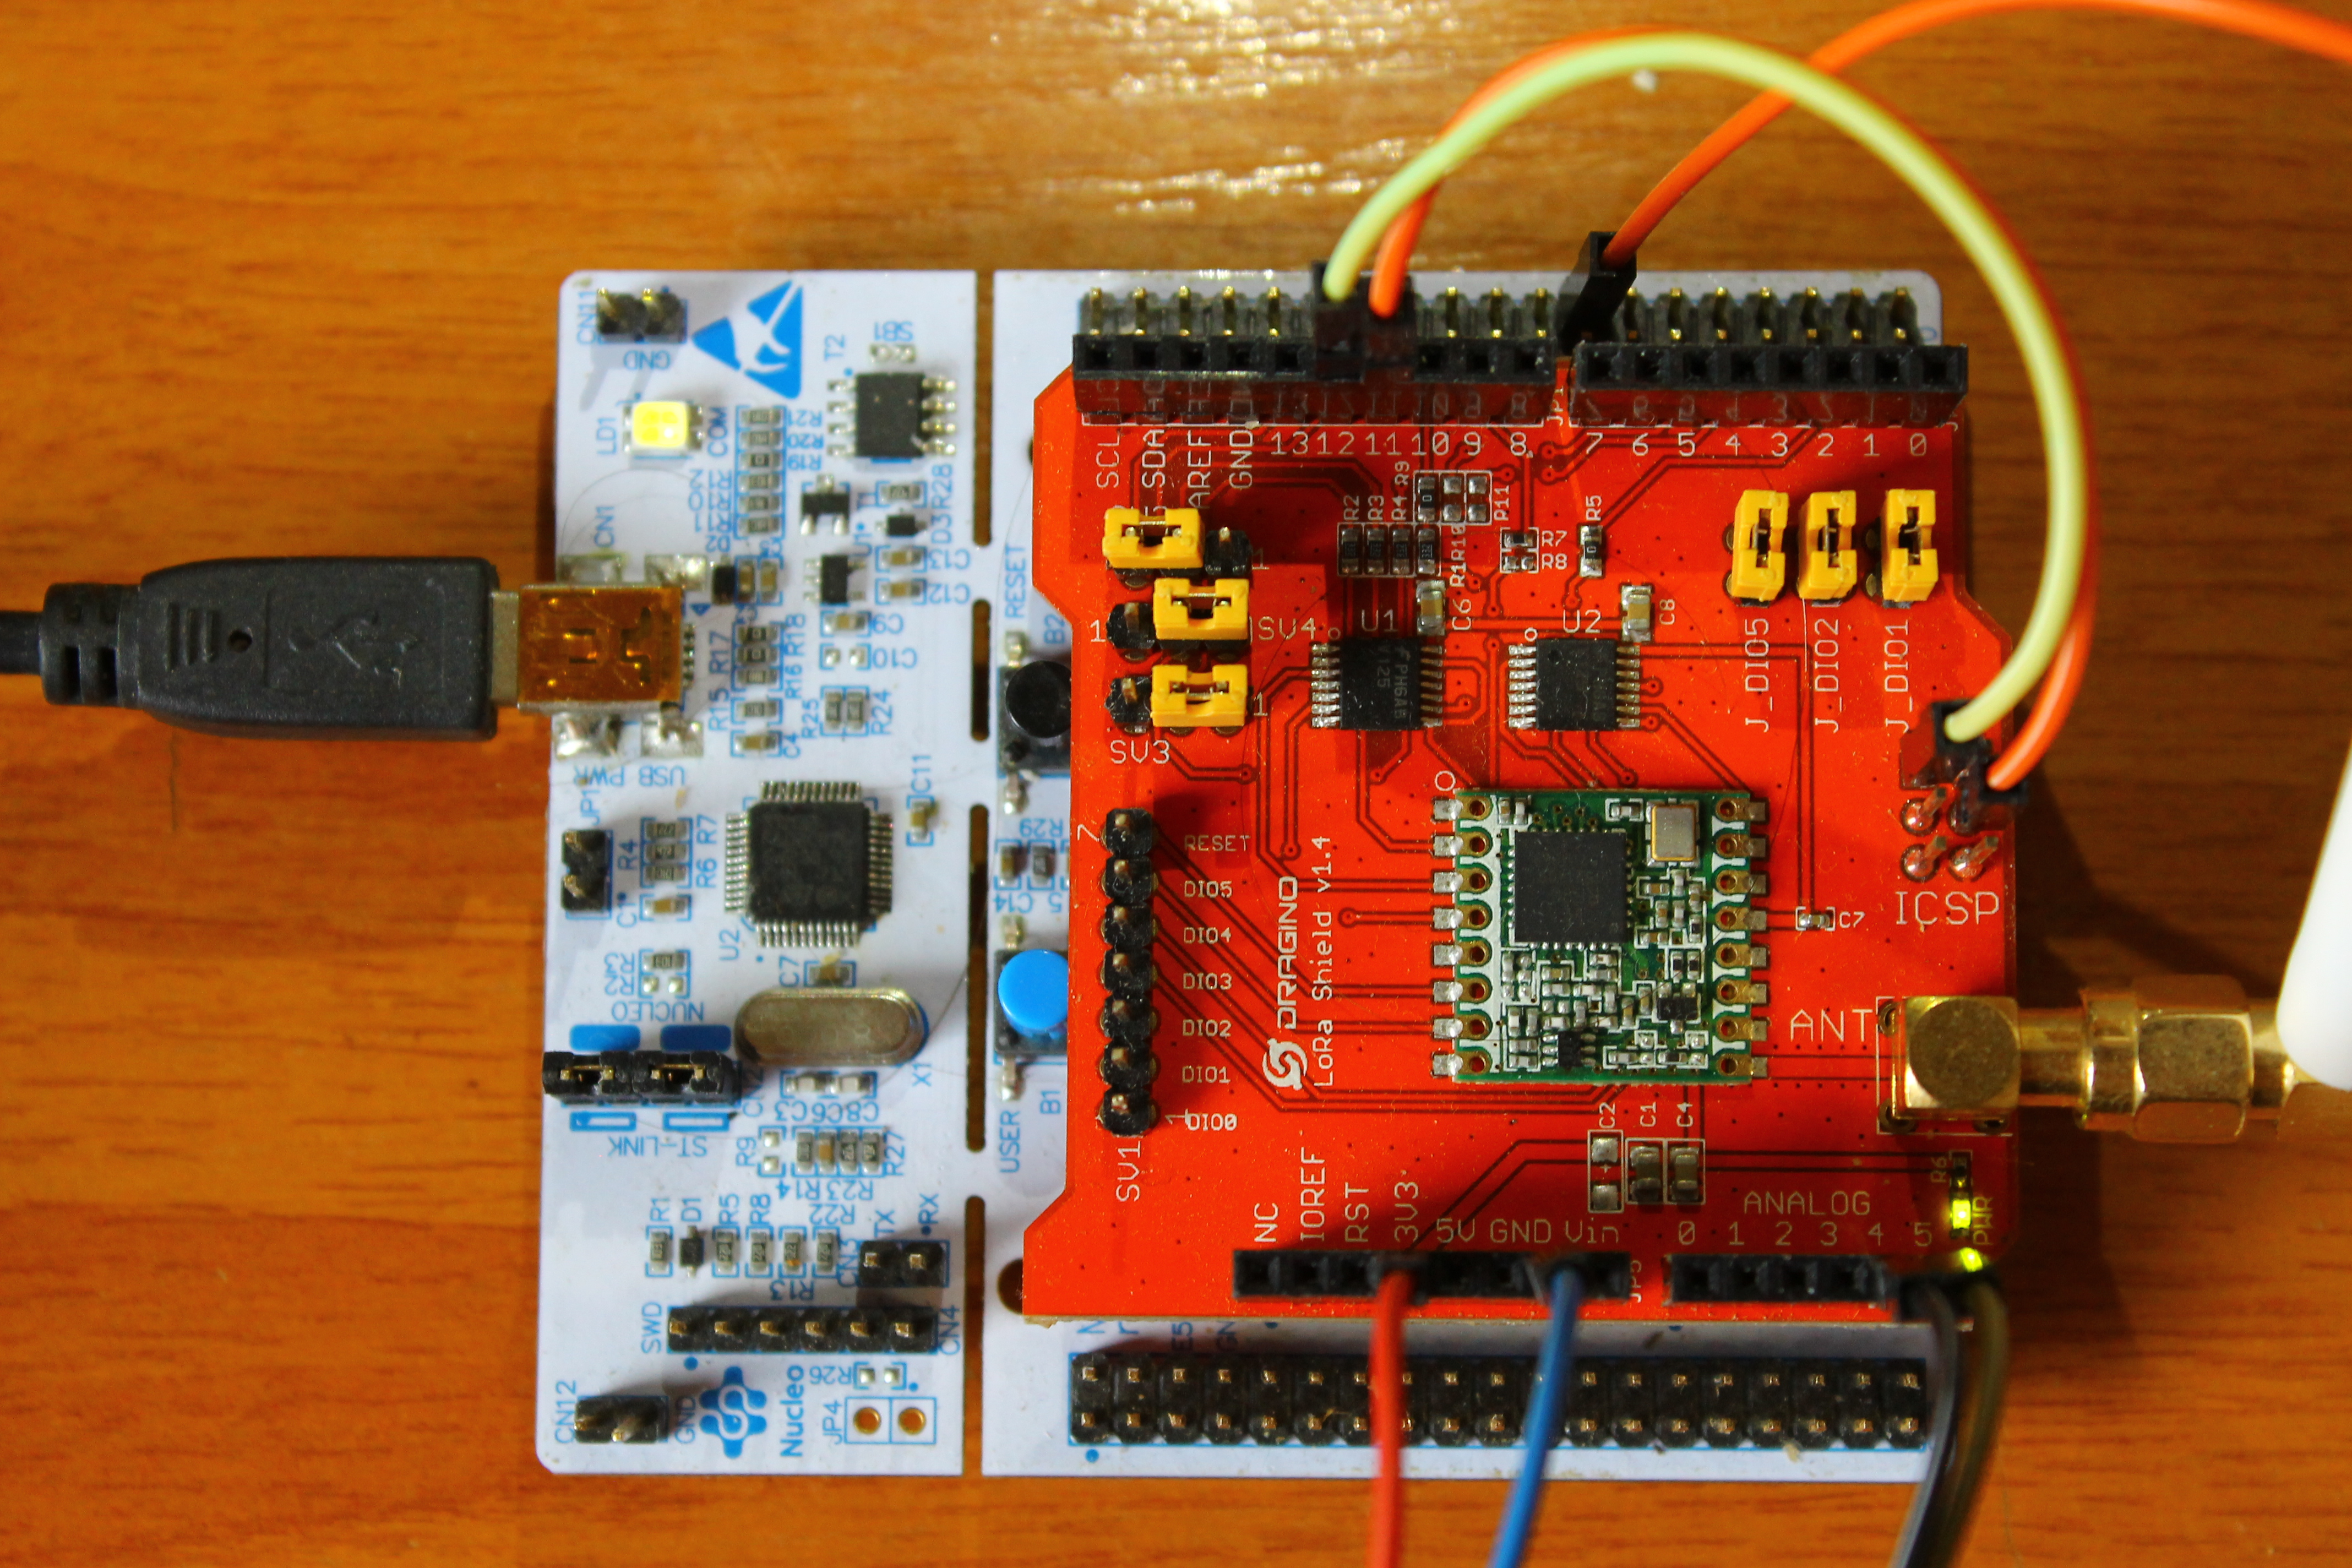
\includegraphics[width=1\textwidth]{foto01}
    \caption{foto zapojení}
    \label{fig:03}
\end{figure}

Pro komunikaci s LoRa transceiverem je tedy použito SPI1, pro komunikaci přes USB je použito USART2 a pro komunikaci přes RS485 je použito UART1.

\begin{table}[h]
    \centering
    \begin{tabular}{ |c|c|c| }
     \hline

     Periférie          & Název pinu & Pin procesoru           \\ \hline \hline
     
                        & RX  &   PC1            \\
    RS485 transceiver   & TX  &   PC0       \\
                        & RTS  &  PB1      \\     \hline

                        & CS    &  PB6             \\
                        & CLK   &  PA5        \\
   LoRa transceiver     & MISO  &  PA6     \\
                        & MOSI  &  PA7        \\
                        & RST   & PC7          \\
                        & DIO0  & PA10         \\
                        \hline

    \end{tabular}
    \caption{Pinout připojení externích periférií k procesoru}
    \label{table:3}
\end{table}

%%%%%%%%%%%%%%%%%%%%%%%%%%%%%%%%%%%%%%%%%%%%%%%%
\section{Naprogramování}
K naprogramování MCU byla použita HAL knihovna a inicializační nástroj STM32CubeMX poskytnuté výrobcem, tedy ST Microelectronics.
Zdrojové soubory programu byly vyvíjeny v textovém editoru VS-Code, ke kompilaci zdrojových souborů byl použit kompilátor arm-none-eabi-gcc a jako pomocný nástroj makefile skript. 

\subsection{Zdrojové soubory projektu}
Pro šifrování LoRaWAN paketu byla použita knihovna AES-128, dostupná na githubu \cite{AESlib} a knihovna OpenPANA také dostupná z githubu \cite{CMAClib}.
Níže je seznam zdrojových souborů.

\begin{figure}[!h]
    \dirtree{%
        .1 Drivers \DTcomment{STM32 Drivers}.
        .1 Inc\DTcomment{Headers}.
            .2 aes.h\DTcomment{AES-128 library for LoRaWAN paket encryption}.
            .2 cmac.h\DTcomment{library for CMAC calculation in LoRaWAN protocol}.
            .2 LinkedList\_ByteArray.h \DTcomment{Byte array linked list library for stacks}.
            .2 LoRaWAN\_paket.h\DTcomment{LoRaWAN library for paket data decoding}.
            .2 stm32l0xx\_hal\_conf.h\DTcomment{HAL initialization of peripherals}.
            .2 ByteArray.h\DTcomment{Library for Byte array operations}.
            .2 LoRa.h\DTcomment{Library for interfacing LoRa transceiver}.
            .2 main.h\DTcomment{Main file}.
            .2 stm32l0xx\_it.h\DTcomment{HAL initialization of peripherals}.
            .2 eeprom.h\DTcomment{Library for eeprom operations}.
            .2 LoRa\_sensors.h\DTcomment{Library for decoding data from payload}.
            .2 rs485\_protocol.h\DTcomment{Library for RS485 IMA protocol}.
            .2 usb.h \DTcomment{Library for USB communication and system configuration}.
        .1 Src\DTcomment{Sources}.
            .2 aes.c \DTcomment{source file to the aes.h}.
            .2 aes.c \DTcomment{source file to the cmac.h}.
            .2 LinkedList\_ByteArray.c \DTcomment{source file to the LinkedList\_ByteArray.h}.
            .2 LoRaWAN\_paket.c  \DTcomment{source file to the LoRaWAN\_paket.h}.
            .2 stm32l0xx\_hal\_msp.c \DTcomment{HAL source file}.
            .2 ByteArray.c  \DTcomment{source file to the ByteArray.h}.
            .2 LoRa.c \DTcomment{source file to the LoRa.h}.
            .2 main.c \DTcomment{main source file}.
            .2 stm32l0xx\_it.c \DTcomment{HAL source file}.
            .2 eeprom.c \DTcomment{source file to the eeprom.h}.
            .2 LoRa\_sensors.c \DTcomment{source file to the LoRa\_sensors.h}.
            .2 rs485\_protocol.c  \DTcomment{source file to the rs485\_protocol.h}.
            .2 system\_stm32l0xx.c \DTcomment{HAL source file}.
            .2 usb.h \DTcomment{source file to the usb.h}.
    }
\end{figure}


\subsection{Nahrání programu do MCU}
Výstupem kompilace je soubor s koncovkou .binary, který je nahrán do MCU. K tomuto nahrání není potřeba žádný speciální SW nebo HW.
Stačí kit připojit k PC přes USB, v PC se kit zobrazí jako flash disk. Zkompilovaný program s koncovkou .binary stačí překopírovat na toto zařízení. 
Po dobu kopírování souboru bliká na kitu LED1 červená/zelená. Jakmile kopírování skončí, program na kitu je spuštěn, případně je možné kit resetovat černým tlačítkem reset.
Pro uvedení Gatewaye do provozu je nutné se připojit k zařízení přes USB a nastavit všechny parametry viz sekce \ref{sec:konfigurace}.  
% \chapter{Measurement Results and Discussion}
\chapter{Testování navrženého řešení}
Tato kapitola zahrnuje testování navržené gatewaye senzorové sítě viz. kapitola \ref{Návrh WSN}, napojené přes síť RS485 na infrastrukturu přístupového systému firmy IMA v univerzítní budově univerzity ČVUT za reálného provozu s připojenými koncovými zařízeními senzorové sítě, které souběžně odesílají data. Ze zachyceného provozu dat v síti RS485 je odhadnut maximální počet připojených koncových zařízení souběžně odesílající data v senzorové síti při zachování správné funkce přístupového systému.

Testování je provedeno v jednom bloku patra univerzity, kde je do jednoho kontrolního panelu připojeno dvanáct CKP zařízení přes síť RS485. Každé z nich ovládá jedny dveře, tedy jednu čtečku a dveřní zámek.
Do této sítě RS485 je navíc připojena navržená gateway jako třinácté CKP zařízení.
K této navržené gatewayi senzorové sítě jsou připojena dvě koncová zařízení typu RHF1S001, dostupné na trhu, vyrbené firmou RisingHF, obsahující senzory teploty a vlhkosti. Pro tento test jsou nakonfigurovány k odesílání dat ze senzorů s intervalem 5 minut.

Gateway a CKP zařízení jsou zapojena dle blokového schematu v obrázku \ref{fig:ACS architecture IMA with geteway}.
Konkrétní rozmístění stávajcích dvanácti CKP zařízení, gatewaye a dvou koncových zařízení senzorové sítě v testovaných prostorách budovy je zobrazeno v obrázku \ref{fig:CorridorFloorPlan}.

\begin{figure*}[!ht]
    \centering
    \includegraphics[width=1\textwidth]{5patro}
    \caption{Rozmístění koncových zařízení sítě a zařízení CKP v testovaných prostorách budovy}
    \label{fig:CorridorFloorPlan}
\end{figure*}

Testování probíhalo od 21. září do 31. října, tedy v době přítomnosti studentů a zaměstnanců v testovaných prostorách. 
Po tuto dobu testování byly zaznamenávány přenášené pakety síti RS485, kontrolní panel přijal 1~876~978 paketů (14~074~522 B) a odeslal 1~101~556 paketů (8~295~219 B), dohromady tedy 2~978~534 paketů (22~369~741 B).
Z naměřených hodnot byla provedena metoda frekvenční analýzy. Z přenesených paketů byly nejdelší 3 o velikostí 40 bytů.
S ohledem na celkové množství paketů je to zanedbatelné množství, tj. 1,3E-04 \%.
Avšak vzhledem k povaze systému, tedy systému s primární funkcí řízení přístupu do omezených oblastí, se za nejhorší scénář považuje nepřekonatelný limit velikosti paketu.

Maximální počet koncových zařízení připojených ke gatewayi při kterém není ovlivněn stávájící přístupový systém je možné vypočítat z rychlosti přenosu dat v síti RS485. 
Tato rezerva rychlosti přenosu dat je uvažována za účelem ochrany přístupového systému před dysfunkcí nebo poruchou, například před dlouhým čekáním na otevření dveří.

\begin{table}[h]
\centering
\footnotesize
\caption{Frekvenční analýza délky paketu}
\begin{ctucolortab}
    \begin{tabular}{|c|r|}
        \hline
Packet length &  Count \\ \hline
\textbf{7}  &  \textbf{2~216~098}  \\
8  &   619~127   \\
9  &         3   \\
11 &    58~393   \\
13 &    58~620   \\
16 &         1   \\
18 &         2   \\
\textbf{19} &    \textbf{26~286}   \\
23 &         1   \\
40 &         3   \\
\hline
\end{tabular}
\end{ctucolortab}
\label{tab:FreqAnalysis}
\end{table}

\begin{figure*}[ht]
    \centering
    \includegraphics[width=1\textwidth]{03-dr-measured}
    \caption{Měřená rychlost přenosu dat [bps] v síti RS485 během doby testování}
    % \caption{Measured data rate in [bps] in RS485 network during long-term operation test}
    \label{fig:PacketLengthMeasuredAll}
\end{figure*}

Na základě frekvenční analýzy uvedené v tabulce \ref{tab:FreqAnalysis} a IMA know-how, pakety přenášející data z koncových zařízení jsou dlouhé 19 bytů a pakety potvrzení IMA protokolu jsou dlouhé 7 bytů. Alespoň dva pakety jsou potřeba k přenesení dat z koncových zařízení přes síť RS485, tj. paket s daty koncového zařízení a paket potvrzení.

V obrázku \ref{fig:PacketLengthMeasuredAll} jsou dvě důležité charakteristiky, maximální délka paketu 
(červená přerušovaná čára) a medián délky paketu (červená nepřerušovaná čára), určeny frekvenční analýzou v tabulce \ref{tab:FreqAnalysis}. 
Průměrné zatížení provozu kanálu sítě RS485 je 6,38 pps, tj. 0,85 Bps.
%shows lengths of captured packet  during
%Median of packet length is determined by using frequency analysis method, as shown in Tab. \ref{tab:FreqAnalysis}.
% 7,51 Byte --> simple arithmetic mean


Z testování provozu jsou zachyceny délky přenášených paketů ($ l $) s časovou přesností na tisícinu sekundy. Údaje o čase jsou převedeny na jednotky sekund pomocí funkce sum, aby byly získány data jako bitová rychlost v bitech za sekundu (bps),
V obrázku \ref{fig:PacketLengthMeasuredAll} červená přerušovaná čára s hodnotou 2520~bps) ukazuje jeden sekundový interval ve kterém součet přenesených paketů v síti RS485.
Na základě podrobných znalosti protokolu IMA se ukazuje, že je využito méně než 20\% kapacity sítě RS485 
%This limit state is caused by data communication of two sensor nodes that occupied 2\% of capacity of used RS485 network.

Aby bylo zabráněno přetížení sítě RS485, maximální počet koncových zařízení připojených ke gatewayi $ S_{MAX} $ je možné vypočítat vztahem:

\begin{equation}
S_{MAX} = \frac{\frac{\frac{v_{485}}{B}}{l_{MAX}} - R}{P}
\label{equ:max-count-of-sensors}
\end{equation}

kde:

\begin{tabular}{l @{  } l}
$v_{485}$ & rychlost přenosu dat v síti RS485 [bps]\\
 B        & počet bitů v bytu (pro přepočítání rychlosti přenosu dat na byty) \\
$l_{MAX}$ & maximální délka paketu \\
 R        & rezerva rychlosti přenosu dat [\%]\\
 P        & počet paketů k přenesení dat z koncového zařízení \\
\end{tabular}


S ohledem na výše uvedené limity, navržené rezervy a rychlosti přenosu dat v síti RS485 je vypočítán maximální počet koncových zařízení senzorové sítě, které souběžně odesílají data přes síť RS485 viz. tabulka \ref{tab:max-sensor-nodes}.

Použité hodnoty pro výpočet jsou:

\begin{tabular}{l @{ $=$ } l}
$v_{485}$ & RS485 network data rate \\
 B        & 8 \\
$l_{MAX}$ & 40 \\
 P        & 2 \\
\end{tabular}

\begin{table}[h]
\centering
\footnotesize
\caption{Maxímální počet připojených koncových zařízení v senzorové síti souběžně odesílající data skrze síť RS485 s určitou rezervou} 
\begin{ctucolortab}
\begin{tabular} {|p{2.5cm}|llll|}
    \hline

\textbf{RS485 rychlost přenosu dat} &       \multicolumn{4}{c|}{\textbf{Rezerva R}}	  	    \\

$v_{485}$ {[bps]}  &	0 \%	&	10 \%	&	20 \%	&	30 \%  \\ \hline

  1200~~~ &    1	&    1	&    1	&    1 \\
  2400~~~ &    3	&    3	&    3	&    2 \\
  4800~~~ &    7	&    6	&    6	&    5 \\
  9600~~~ &   15	&   13	&   12	&   10 \\
 19200~~~ &   30	&   27	&   24	&   21 \\
 38400~~~ &   60	&   54	&   48	&   42 \\
 57600~~~ &   90	&   81	&   72	&   63 \\
115200~~~ &  180	&  162	&  144	&  126 \\
230400~~~ &  360	&  324	&  288	&  252 \\
460800~~~ &  720	&  648	&  576	&  504 \\
921600~~~ & 1440	& 1296	& 1152	& 1008 \\
\hline

\end{tabular}
\end{ctucolortab}

\label{tab:max-sensor-nodes}
\end{table}


Např. v senzorové síti může být až 54 koncových zařízení připojených ke gatewayi, která je napojena na síť RS485 s přenosovou rychlostí 38400~bps a rezervou 10 \% nebo 42 koncových zařízení s přenosovou rychlostí 38400~bps a rezervou 30 \%.
Tento výsledek ukazuje, že jeden blok patra univerzity, tj. jedna síť RS485 je schopna fungovat s desítkami koncovými zařízeními senzorové sítě souběžně vysílající data s dostatečnou rezervou chránící přístupový systém. 






%%%%%%%%%%%%%%%%%%%%%%%%%%%%%%%%%%%%%%%%%%%%%%%%%%%%%%%%%%%%%%%%%%%%%%%%%%%%%%%%%%%%%%%
%       NOT USED
%%%%%%%%%%%%%%%%%%%%%%%%%%%%%%%%%%%%%%%%%%%%%%%%%%%%%%%%%%%%%%%%%%%%%%%%%%%%%%%%%%%%%%%
% The heavy traffic test simulates data transmission in the RS485 network as evidence of theoretically calculated values as shown in Tab \ref{tab:max-sensor-nodes}.

% \begin{figure}[!ht]
    % \centering
    % \includegraphics[width=.5\textwidth]{03-tp-simul}
    % \caption{RS485 datarates in simulation of heavy data traffic}
    % \label{fig:heavySimulation}
% \end{figure}

% This test simulated the transmission of more than 190~000 commands from 300 sensor nodes every 5 minutes simultaneously for 12 hours time period. The highest datarate achieved during simulation is 1160~bps, Fig \ref{fig:heavySimulation} red dashed line.

%!!! Tady to mozna chce frekvencni analyzu GW, at vis, jak jsou dlouhe pakety, pak nemusis hadat, nebo napis, ze max. delka je 19 bytů.

%Considering the worst case, ie packets with length of 40 Bytes, we have analytically calculated the maximum number of sensors a network can transmit based on the network transmission rate.

%\textbf{!!! Limit RS485: up to 32 transceivers on the serial bus !!! My vsak mame senzory pres LoRa ...Jo, ale to je fyzicky, to splnujeme, mame jich 13 :-)}
%datasheet: https://www.sparkfun.com/datasheets/Components/General/sp3485CN-LTR.pdf

%Space for peaks 10\% --> maximum packet rate is 324 pps
%Data measured in testing procedure shows Fig.

%\begin{table}[h]
%\centering
%\footnotesize
%\caption{Simple analytics of measured data}
%\begin{tabular}{lr}
%\textbf{Packet length} & \textbf{Bytes} \\ \hline
%Minimum   &   7 B     \\
%Maximum   &  40 B     \\
%mean      &   7,51 B  \\
%Median    &   7 B     \\
%\end{tabular}
%\label{tab: simple-analytics}
%\end{table}


%---
% tabulka, rezervy 10%, 30% ...
% Zjistit kolik sensoru muze byt na sbernici 485.
% popis os co  je co

\chapter{Návrh vylepšení systému}
\label{Návrh vylepšení systému}
V této kapitole jsou navrženy způsoby vylepšení navrženého systému.


% \section{Možnosti odstranění omezení navržené gatewaye - závislost na znalosti typu koncových zařízení senzorové sítě}
\section{Vylepšení infrastruktury systému}
Jedním z největších omezení navrženého systému je, že FW gatewaye musí podporovat typy koncových zařízení senzorové sítě, aby na základě typu koncového zařízení byl správně zpracován jeho payload.
Přidání nového typu zařízení do sítě vyžaduje update FW gatewaye.
Aby gateway nebyla závislá na znalosti typu koncových zařízení senzorové sítě, je potřeba přenášet celý aplikační payload koncových zařízení přes síť RS485, což má nežádoucí důsledek a to zvýšení objemu přenášených dat v síti RS485 přístupového systému.
Původní navržené řešení viz. kapitola \ref{Návrh senzorové sítě} totiž klade důraz na nízký objem přenášených dat v síti RS485.

Například použitý typ koncového zařízení RHF1S001 \ref{sec:RHF1S001} odesílá LoRaWAN pakety o délce 22 bytů, z toho je 9 bytů aplikační payload. Protokol umožňuje posílat pakety o velikosti až 256 bytů, z toho je nejméně 13 bytů data protokolu, tedy maximální délka aplikačního payloadu může být až 243 bytů.

Efektivní řešení by bylo rozšíření CKP protokolu sítě RS485 přístupového sytému o nový typ příkazu umožňující odeslat paket o maximální délce payloadu až 243 bytů, tedy aby jedním tímto paketem bylo možné odeslat celý aplikační payload. 
Je zde bezpečnostní výhoda, že aplikační payload by pak mohl být dešifrován až na serveru LoRaWAN klíčem AppSKey, tudíž data z koncových zařízení by nebyla odhalitelná v síti RS485.
Toto řešení tedy vyžaduje update FW všech kontrolních panelů, což je velmi náročné.
% tudíž realizace tohot řešení prozatím neni plánována.

Nicméně je možné implementovat podobné řešení bez nutnosti zavádění nového typu paketu pro aplikační payload koncového zařízení senzorové sítě tak, že aplikační payload by byl rozdělen a odeslán posloupností několika paketů průchod. 
Např. z dostupných 6 bytů v jednom paketu průchod by jeden byte obsahoval informaci o čísle paketu dané sekvence a zbylých 5 bytů by byly data payloadu daného koncového zařízení Zařízení typu RHF1S001, které má aplikační payload o velikosti 9 bytů by byl takto odeslán dvěma pakety průchod. Jelikož každý paket průchod je potvrzován, toto řešení by rapidně zvýšilo objem přenášených dat v síti RS485.



%%%%%%%%%%%%%%%%%%%%%%%%%%%%%%%%%%%%%%%%%%%%%%%%%%%%%%
\section{Vylepšení navržené gatewaye}
U původního realizovaného prototypu gatewaye jsou komponenty propojovány drátkama, tudíž mohlo dojít k rozpojení při manipulaci se zařízením. 
V tomto provedení prototypu by bylo náročné vyrobit několik jednotek až desítek kusů pro případné zákazníky.
Jako další nevýhody původního prototypu jsou, že zařízení je zbytečně velké, nemá napěťové ochrany, a v RS485 transceiveru byl na pevno napájen odpor impedancniho zakonceni site RS485.
Z těchto důvodů je navržena a realizována verze 2 s plošným spojem (PCB) navrženým v Eagle.
Schéma zapojení je v obrázku \ref{fig:minigateway_schema} a plošný spoj je v obrázku \ref{fig:minigateway_plosnak}.
Je zde použit jiný vývojový kit NUCLEO-L432KC \cite{nucleo-l432KC_ST} s výkonnějším procesorem STM32L432KC, jehož parametry jsou v tabulce \ref{tab:mcuFeatures_stm43l432kc}. 

\begin{longtable}{|l|p{3.5cm}|}
    \caption{Vlastnosti mikrokontroléru STM32L432KC \cite{nucleo-l432KC_ST}}
    \label{tab:mcuFeatures_stm43l432kc} \\
    \hline

    Parametr          & Informace            \\ \hline \hline

    Architektura mikrokontroléru & ARM Cortex-M4 32-bit RISC \\ \hline
    Interní paměť flash       & 256 KB \\ \hline
    Interní paměť RAM         & 64 kB \\ \hline
    Frekvence CPU               & up to 80 MHz \\ \hline
    Rozhranní                  & 2x SPI, 2x I2C, 3x UART, 1x CAN, 1x SWP \\ \hline

\end{longtable}

Použitý procesor STM32L432KC neobsahuje paměť EEPROM, tudíž jako non-volatile paměť pro ukládání konfigurace je použita paměť flash.
Použitý vývojový kit NUCLEO-L432KC má pinout stejný jako Arduino Nano, tedy je pod tímto názvem ve schématu.
LoRa transceiver je použit RFM95w \cite{RFM95w} bez shieldu.
RS485 transceiver je použit LTC1480. 
Do zařízení je dále přidán externí stabilizátor, napěťový filtr, impedanční zakončení sítě RS485 přes přepínač a napěťové ochrany pro linky A, B a napájení. 
Připojení periférií k GPIO mikrokontroléru je znázorněno v tabulce \ref{table:Pinout připojení periférií k mikrokontroléru v2}.

\newpage
\begin{longtable}{ |c|c|c| }

    \caption{Pinout připojení periférií k mikrokontroléru}
    \label{table:Pinout připojení periférií k mikrokontroléru v2} \\
\hline

Periférie          & Název pinu & GPIO mikrokontroléru           \\ \hline \hline

            & CS    &  PB6             \\
            & CLK   &  PA5        \\
LoRa transceiver    & MISO  &  PA6     \\
            & MOSI  &  PA7        \\
            & RST   & PC7          \\
            & DIO0  & PA10         \\
            \hline

            & RX  &   PC1            \\
RS485 transceiver   & TX  &   PC0       \\
            & RTS  &  PB1      \\     \hline

USB konektor        & RX    & PA3    \\
            & TX    & PA2   \\          \hline
\end{longtable}


\begin{figure}[!h]
    \centering
    \includegraphics[width=1\textwidth]{minigateway_schema}
    \caption{Návrh gatewaye verze 2 - schéma}
    \label{fig:minigateway_schema}
\end{figure}

\begin{figure}[!h]
    \centering
    \includegraphics[width=0.7\textwidth]{minigateway_plosnak}
    \caption{Návrh gatewaye verze 2 - plošný spoj}
    \label{fig:minigateway_plosnak}
\end{figure}


Dle návrhu byla gateway realizována viz foto \ref{fig:minigateway_fotoV2}.

\begin{figure}[!h]
    \centering
    \includegraphics[width=0.6\textwidth]{photo_minigatewayV2}
    \caption{Foto gatewaye verze 2}
    \label{fig:minigateway_fotoV2}
\end{figure}




\chapter{Závěr}
V této práci jsou diskutovány podmínky rozšíření stávajícího přístupového systému pracujícího s průmyslově standardizovanou sítí RS485 o bezdrátovou senzorovou síť založenou na LoRaWAN protokolu v jednokanálovém módu.
Dále je takováto senzorová síť navržena a realizována vytvořením prototypu jednokanálové LoRaWAN gatewaye připojené do sítě RS485 infrastruktury přístupového systému, kde jsou připojeny tzv. CKP zařízení ovládající dveřní zámky a čtečky, komunikující vlastním proprietárním CKP protokolem, který podoruje i navržená gateway.
K navržené gatewayi jsou připojeny LoRaWAN senzory třetích stran jako koncová zařízení senzorové sítě.
Na univerzitě, kde je tento přístupový systém zaveden, je proveden test dlouhodobého provozu. Při tomto testu je navržená gateway připojena do jedné sítě RS485, která již obsahje 12 CKP zařízení (páry čteček a dveřních zámků) a ke gatewayi jsou připojena dva LoRaWAN senzory jako koncová zařízení senzorové sítě.
Během doby testování jsou zaznamenávány přenášené pakety v síti RS485.
Ze zaznamenaných dat je provedena frekvenční analíza délek paketů, a je vypočítán maximální počet koncových zařízení senzorové sítě souběžně odesílajících data, v závislosti na rychlosti přenosu dat v síti RS485 a rezervě přenosové rychlosti, pro zachování správné funkce přístupového systému.
Např. do sítě RS485 s přenosovou rychlostí 38400 bps, s rezervou 20 \% je možné připojit navrženou gatewaye senzorové sítě a k ní připojit až 48 koncových zařízení, což je dostačující pro systémy bezdrátového měření.




% a je zvažována největší hodnota délky paketu, stejně jako rezerva rychlosti přenosu dat v síti RS485 za účelem ochrany správné funkcionality systému řízení přístupu.
% Frequency analysis of packet lengths is performed and the biggest value of packet length is considered as well as the reserve of the RS485 data rate in order to protect the access control system from malfunction. 

% Z nměřených dat je vypočítán maximální počet koncových zařízení senzorové sítě souběžně odesílajících data, v závislosti na rychlosti přenosu dat v síti RS485 a rezervě přenosové rychlosti, např 81 koncových zařízení připojených ke gatewayi senzorové sítě, napojené do sítě RS485 s přenosovou rychlostí 57600~bps a 10 \% rezervou. 
% This number of sensor nodes significantly exceeds the actual needs of the sensor nodes on one floor block of university building. Therefore we can state that WSN is suitable for smart metering applications.




%%%%%%%%%%%%%%%%%%%%%%%%%%%%%%%%%%%%%%%%%%%%%%%%
\bibliographystyle{amsalpha}
\bibliographystyle{csn690}
\bibliography{mybibliographyfile}
\begin{thebibliography}{9}
%%%%%%%%%%%%%%%%%%%%%%%%%%%%%%%%%%%%%%%%%%%%%%%%%%%%%%%%%%%%%%%



% % -------------------------
\bibitem[1]{Design and Implementation of an IoT Assisted Real Time ZigBee Mesh WSN}
H. Ali, W. Y. Chew, F. Khan and S. R. Weller, "Design and implementation of an IoT assisted real-time ZigBee mesh WSN based AMR system for deployment in smart cities," \textit{2017 IEEE International Conference on Smart Energy Grid Engineering (SEGE)}, Oshawa, ON, 2017, pp. 264-270.
[Online]. Available:
\url{
https://ieeexplore.ieee.org/stamp/stamp.jsp?tp=&arnumber=8052810
}
[Accessed: 9-Sep-2019].


% % % -------------------------
\bibitem[2]{Internet of Things (IoT) for building Smart Home System}
T. Malche and P. Maheshwary, "Internet of Things (IoT) for building smart home system," \textit{2017 International Conference on I-SMAC (IoT in Social, Mobile, Analytics and Cloud) (I-SMAC)}, Palladam, 2017, pp. 65-70.
[Online]. Available:
\url{
https://ieeexplore.ieee.org/stamp/stamp.jsp?tp=&arnumber=8058258
}
[Accessed: 9-Sep-2019].


% % -------------------------
\bibitem[3]{A comparative study of LPWAN technologies for large-scale IoTdeployment}
K. Mekki, E. Bajic, F. Chaxel and F. Meyer, "A comparative study of LPWAN technologies for large-scale IoT deployment". \textit{ICT Express}, vol. 5, no. 1, March 2019.
[Online]. Available:
\url{
https://www.sciencedirect.com/science/article/pii/S2405959517302953
}
[Accessed: 9-Sep-2019].

% % -------------------------
\bibitem[4]{Long-Range Communications in Unlicensed Bands}
M. Centenaro, L. Vangelista, A. Zanella and M. Zorzi, "Long-range communications in unlicensed bands: the rising stars in the IoT and smart city scenarios," in \textit{IEEE Wireless Communications}, vol. 23, no. 5, pp. 60-67, October 2016.
[Online]. Available:
\url{
https://ieeexplore.ieee.org/stamp/stamp.jsp?tp=&arnumber=7721743
}
[Accessed: 9-Sep-2019].

% -------------------------
\bibitem[5]{high density LPWAN}
A. Lavric and A. loan Petrariu, "High-Density Low Power Wide Area Networks," \textit{2018 10th International Conference on Electronics, Computers and Artificial Intelligence (ECAI)}, Iasi, Romania, 2018, pp. 1-4.
[Online]. Available:
\url{
https://ieeexplore.ieee.org/stamp/stamp.jsp?tp=&arnumber=8678997
}
[Accessed: 9-Sep-2019].

% % -------------------------
\bibitem[6]{MURS Band for LPWAN Applications}
A. Kosari and D. D. Wentzloff, "MURS Band for LPWAN Applications," \textit{2019 IEEE Topical Conference on Wireless Sensors and Sensor Networks (WiSNet)}, Orlando, FL, USA, 2019, pp. 1-3.
[Online]. Available:
\url{
https://ieeexplore.ieee.org/stamp/stamp.jsp?tp=&arnumber=8711814
}
[Accessed: 9-Sep-2019].


% -------------------------
\bibitem[7]{IoT cisco study}
KRANZ, Maclej. The Internet of Things: 5 Predictions for 2018. CISCO: blog 
[Online]. Available:
\url{
https://blogs.cisco.com/innovation/the-internet-of-things-5-predictions-for-2018
}
[Accessed: 9-Sep-2019].

% % -------------------------
\bibitem[8]{Flexible Wireless Sensor Network for smart lighting applications}
R. F. Fernandes, C. C. Fonseca, D. Brandão, P. Ferrari, A. Flammini and A. Vezzoli, "Flexible Wireless Sensor Network for smart lighting applications," 2014 IEEE International Instrumentation and Measurement Technology Conference (I2MTC) Proceedings, Montevideo, 2014, pp. 434-439.
[Online]. Available:
\url{
https://ieeexplore.ieee.org/stamp/stamp.jsp?tp=&arnumber=6860782
}
[Accessed: 9-Sep-2019].



% % % -------------------------
\bibitem[9]{Building a Smart Home System with WSN and Service Robot}
W. Huiyong, W. Jingyang and H. Min, "Building a Smart Home System with WSN and Service Robot," \textit{2013 Fifth International Conference on Measuring Technology and Mechatronics Automation}, Hong Kong, 2013, pp. 353-356.
[Online]. Available:
\url{
https://ieeexplore.ieee.org/stamp/stamp.jsp?tp=&arnumber=6493740
}
[Accessed: 9-Sep-2019].


% % -------------------------
\bibitem[10]{A Meter Reading System Based on WSN}
Luo Hui, "A meter reading system based on WSN," \textit{2010 International Conference on Optics, Photonics and Energy Engineering (OPEE)}, Wuhan, 2010, pp. 311-314.
[Online]. Available:
\url{
https://ieeexplore.ieee.org/stamp/stamp.jsp?tp=&arnumber=5508121
}
[Accessed: 9-Sep-2019].


% % -------------------------
\bibitem[11]{Smart Water Meter System for User-Centric Consumption Measurement}
M. J. Mudumbe and A. M. Abu-Mahfouz, "Smart water meter system for user-centric consumption measurement," \textit{2015 IEEE 13th International Conference on Industrial Informatics (INDIN)}, Cambridge, 2015, pp. 993-998.
[Online]. Available:
\url{
https://ieeexplore.ieee.org/stamp/stamp.jsp?tp=&arnumber=7281870
}
[Accessed: 9-Sep-2019].


% % -------------------------
\bibitem[12]{Radio Data Infrastructure for Remote Monitoring}
R. K. Kodali, "Radio data infrastructure for remote monitoring system using lora technology," \textit{2017 International Conference on Advances in Computing, Communications and Informatics (ICACCI)}, Udupi, 2017, pp. 467-472.
[Online]. Available:
\url{
https://ieeexplore.ieee.org/stamp/stamp.jsp?tp=&arnumber=8125884
}
[Accessed: 9-Sep-2019].


% % -------------------------
\bibitem[13]{Smart Electric Meter Using LoRA Protocols and Iot applications}
N. Shah and P. S. Sundar, "Smart Electric Meter Using LoRA Protocols and lot applications," \textit{2018 Second International Conference on Electronics, Communication and Aerospace Technology (ICECA)}, Coimbatore, 2018, pp. 1178-1180.
[Online]. Available:
\url{
https://ieeexplore.ieee.org/stamp/stamp.jsp?tp=&arnumber=8474749
}
[Accessed: 9-Sep-2019].



% % -------------------------
\bibitem[14]{ttn}
The Things Network, TODO
[Online]. Available:
\url{
https://www.thethingsnetwork.org/
}
[Accessed: 25-Apr-2020].



% % -------------------------
\bibitem[15]{Implement Smart Farm with IoT Technology}
C. Yoon, M. Huh, S. Kang, J. Park and C. Lee, "Implement smart farm with IoT technology," \textit{2018 20th International Conference on Advanced Communication Technology (ICACT)}, Chuncheon-si Gangwon-do, Korea (South), 2018, pp. 749-752.
[Online]. Available:
\url{
https://ieeexplore.ieee.org/stamp/stamp.jsp?tp=&arnumber=8323908
}
[Accessed: 9-Sep-2019].



% -------------------------
% -------------------------
% -------------------------


% -------------------------
\bibitem[16]{accessControlSystem_eiprocus}
Know about Access Control Systems and Their Types with Features. \textit{Electronics projects focus}
[Online]. Available:
\url{
https://www.elprocus.com/understanding-about-types-of-access-control-systems/
}
[Accessed: 9-Sep-2019].



% -------------------------
% -------------------------
% -------------------------



%___________________
%% notused
\bibitem[17]{iqrf_rf}
\textit{
RF.
}
IQRF Alliance.

[Online]. Available:
\url{
https://www.iqrf.org/technology/rf
}
[Accessed: 9-Jun-2018].



%___________________
%% notused
\bibitem[18]{iqrf_ide}
\textit{
IQRF IDE
}
IQRF Alliance.

[Online]. Available:
\url{
https://www.iqrf.org/technology/iqrf-ide
}
[Accessed: 9-Jun-2018].



%___________________

\bibitem[19]{iqrf_sdk}
\textit{
IQRF SDK.
}
IQRF Alliance.
[Online]. Available:
\url{
https://www.iqrf.org/technology/iqrf-sdk
}
[Accessed: 9-Jun-2018].

%___________________


\bibitem[20]{iqrf_transceivers}
\textit{
Transceivers.
}
IQRF Alliance.

[Online]. Available:
\url{
https://www.iqrf.org/products/transceivers
}
[Accessed: 9-Jun-2018].

%___________________

\bibitem[21]{iqrf_alliance}
\textit{
Three security levels in new IQRF OS 4.0.
}
IQRF Alliance.
[Online]. Available:
\url{
https://www.iqrfalliance.org/news/117-three-security-levels-in-new-iqrf-os-4-0
}
[Accessed: 9-Jun-2018].


\bibitem[22]{paper_iqrf}

[Online]. Available:
\url{
https://ieeexplore.ieee.org/stamp/stamp.jsp?tp=&arnumber=8399666
}
[Accessed: 9-Sep-2019].


%___________________ Wireless M-Bus

\bibitem[23]{EN 13757}
[Online]. Available:
\url{
https://ec.europa.eu/eip/ageing/standards/ict-and-communication/data/en-13757_en
}
[Accessed: 2-Apr-2020].


\bibitem[24]{wirelessMBus_automatizace}
[Online]. Available:
\url{
https://automatizace.hw.cz//sbernice-wireless-mbus-jde-i-bezdratove
}
[Accessed: 9-Jun-2018].

%___________________

\bibitem[25]{wirelessMBus01}
\textit{
Wireless Meter Bus, WM-Bus Technology.
}
Radio-Electronics.
[Online]. Available:
\url{
http://www.radio-electronics.com/info/wireless/wireless-m-bus/basics-tutorial.php
}
[Accessed: 9-Jun-2018].

%___________________

\bibitem[26]{wirelessMBus02}
\textit{
Wireless M-Bus in Industrial Wireless Sensor Networks.
}
Radiocrafts.
[Online]. Available:
\url{
https://radiocrafts.com/technologies/wireless-m-bus-technology-overview/
}
[Accessed: 9-Jun-2018].

%___________________

% page unavailable
% \bibitem[24]{7}
% Radiocrafts: 
% \textit{
% WirelessM-Bus in Industrial Sensor Networks.
% }
% [Online]. Available:
% \url{
% https://radiocrafts.com/uploads/AN024_Using_Wireless_M-BUS_in_Industrial_Sensor_Networks_1_0.pdf
% }
% [Accessed: 9-Jun-2018].

%___________________

\bibitem[27]{wirelessMBus03}
Silicon labs: 
\textit{
WIRELESS M-BUS SOFTWARE IMPLEMENTATION.
}
[Online]. Available:
\url{
https://www.silabs.com/documents/public/application-notes/AN451.pdf
}
[Accessed: 9-Jun-2018].

%___________________

\bibitem[28]{wirelessMBus04}
Compass security:
\textit{
Wireless M-Bus Security Whitepaper Black Hat USA 2013.
}
June 30th. 2013, v1.01.
[Online]. Available:
\url{
https://www.compass-security.com/fileadmin/Datein/Research/Praesentationen/blackhat_2013_wmbus_security_whitepaper.pdf
}
[Accessed: 9-Jun-2018].


% % % -------------------------
% \bibitem[1118]{ZigBee-based Vehicle Access Control System}

% [Online]. Available:
% \url{
% https://ieeexplore.ieee.org/stamp/stamp.jsp?tp=&arnumber=5453569
% }
% [Accessed: 9-Sep-2019].


%___________________

% \bibitem[27]{Zigbee_wiki}
% \textit{
% Zigbee.
% }
% Wikipedia.
% [Online]. Available:
% \url{
% https://en.wikipedia.org/wiki/Zigbee
% }
% [Accessed: 9-Jun-2018].

%___________________


% \bibitem[28]{Zigbee_mit}
% Xueqi Fan, Fransisca Susan, William Long, Shangyan Li: 
% \textit{
% Security Analysis of Zigbee.
% }
% May 18, 2017.
% [Online]. Available:
% \url{
% https://courses.csail.mit.edu/6.857/2017/project/17.pdf
% }
% [Accessed: 9-Jun-2018].

%___________________


\bibitem[29]{Zigbee_alliance_about}
\textit{
The Zigbee Alliance.
}
Zigbee alliance.
[Online]. Available:
\url{
http://www.zigbee.org/zigbee-for-developers/about-us/
}
[Accessed: 9-Jun-2018].

%___________________


\bibitem[30]{Zigbee_alliance_solution}
\textit{
The Zigbee Alliance.
}
Zigbee alliance.
[Online]. Available:
\url{
https://zigbeealliance.org/solution/zigbee/
}
[Accessed: 9-Jun-2018].

%___________________ Bluetooth LE

% \bibitem[30]{13}
% \textit{
% Bluetooth sensor network.
% }
% mikroelektronika.
% [Online]. Available:
% \url{
% https://www.mikroe.com/blog/bluetooth-sensor-network
% }
% [Accessed: 9-Jun-2018].

% %___________________


% \bibitem[31]{14}
% \textit{
% Dispelling Common Bluetooth Misconceptions.
% }
% Sans technology institute.
% [Online]. Available:
% \url{
% https://www.sans.edu/cyber-research/security-laboratory/article/bluetooth
% }
% [Accessed: 9-Jun-2018].

% %___________________


% \bibitem[32]{15}
% \textit{
% Bluetooth radio interface, modulation, \& channels.
% }
% Radioelectronics.
% [Online]. Available:
% \url{
% http://www.radio-electronics.com/info/wireless/bluetooth/radio-interface-modulation.php
% }
% [Accessed: 9-Jun-2018].

% %___________________


% \bibitem[33]{16}
% Kianoosh Karami: 
% \textit{
% BLE Packet.
% } Punch through.  November 07 2016.  
% [Online]. Available:
% \url{
% https://punchthrough.com/blog/posts/maximizing-ble-throughput-part-2-use-larger-att-mtu
% }
% [Accessed: 9-Jun-2018].


\bibitem[31]{BT_alliance}
\textit{
BLE Packet.
}
[Online]. Available:
\url{
https://www.bluetooth.com/learn-about-bluetooth/bluetooth-technology/radio-versions/
}
[Accessed: 9-Jun-2018].


\bibitem[32]{BT_nordic}
\textit{
BLE Packet.
}
[Online]. Available:
\url{
https://blog.nordicsemi.com/getconnected/things-you-should-know-about-bluetooth-range
}
[Accessed: 9-Jun-2018].

%___________________ LoRa



% \bibitem[2217]{17}
% \textit{
% LoRa Wireless for M2M \& IoT.
% }
% Radioelectronics.
% [Online]. Available:
% \url{
% http://www.radio-electronics.com/info/wireless/lora/basics-tutorial.php
% }
% [Accessed: 9-Jun-2018].

% \bibitem[2218]{18}
% \textit{
% LoRa Network: LoRaWAN.
% }
% Radioelectronics.
% [Online]. Available:
% \url{
% http://www.radio-electronics.com/info/wireless/lora/lorawan-network-architecture.php
% }
% [Accessed: 9-Jun-2018].

\bibitem[33]{lorawan_specification}
LoRa Alliance, "LoRaWAN 1.1 Specification", version 1.1, October 11, 2017
[Online]. Available:
\url{
https://lora-alliance.org/sites/default/files/2018-04/lorawantm_specification_-v1.1.pdf
}
[Accessed: 9-Sep-2019].

% \bibitem[32]{lorawan_limits}
% \textit{
% Understanding the Limits of LoRaWAN.
% } IEEE.
% Communications Magazine. January 2017
% [Online]. Available:
% \url{
% https://arxiv.org/pdf/1607.08011.pdf
% }
% [Accessed: 9-Jun-2018].

% \bibitem[2220]{20}
% BRIAN RAY: 
% \textit{
% Use Cases and Considerations for LoRaWAN.
% }
% Link-labs. June 20, 2016.
% [Online]. Available:
% \url{
% https://www.link-labs.com/blog/use-cases-and-considerations-for-lorawan
% }
% [Accessed: 9-Jun-2018].

% \bibitem[2221]{21}
% \textit{
% LoRa Physical Layer \& RF Interface.
% }
% Radioelectronics.
% [Online]. Available:
% \url{
% http://www.radio-electronics.com/info/wireless/lora/rf-interface-physical-layer.php
% }
% [Accessed: 9-Jun-2018].

% \bibitem[2222]{22}
% Kianoosh Karami: 
% \textit{
% BLE Packet
% }
% Punch through. November 07, 2016.
% [Online]. Available:
% \url{
% https://punchthrough.com/blog/posts/maximizing-ble-throughput-part-2-use-larger-att-mtu
% }
% [Accessed: 9-Jun-2018].

% \bibitem[2223]{23}
% \textit{
% Build your own gateway.
% }
% The things network.
% [Online]. Available:
% \url{
% https://www.thethingsnetwork.org/docs/gateways/start/build.html
% }
% [Accessed: 9-Jun-2018].

% \bibitem[2224]{24}
% \textit{
% LoraWAN in Europe.
% }
% Match X.
% [Online]. Available:
% \url{
% https://matchx.io/community/eu/12-lorawan-in-europe
% }
% [Accessed: 9-Jun-2018].

%________________________________________ Z-Wave

% \bibitem[32]{27}
% \textit{
% Z-Wave.
% }
% Z-wawe Alliance.
% [Online]. Available:
% \url{
% http://www.z-wave.com/about
% }
% [Accessed: 9-Jun-2018].


% \bibitem[33]{28}
% \textit{
% Z-Wave.
% }
% Wikipedia.
% [Online]. Available:
% \url{
% https://en.wikipedia.org/wiki/Z-Wave
% }
% [Accessed: 9-Jun-2018].


% %____________________________________________ Sigfox

% \bibitem[2225]{25}
% Ian Poole: 
% \textit{
% SIGFOX for M2M \& IoT.
% }
% Radioelektronics.
% [Online]. Available:
% \url{
% http://www.radio-electronics.com/info/wireless/sigfox/basics-tutorial.php
% }
% [Accessed: 9-Jun-2018].

% \bibitem[2226]{26}
% \textit{
% SIGFOX for white paper security.
% }
% Sigfox. February 2017.
% [Online]. Available:
% \url{
% https://www.sigfox.com/sites/default/files/1701-SIGFOX-White_Paper_Security.pdf
% }
% [Accessed: 9-Jun-2018].


% %__________________________________________________________ Thread

% \bibitem[2229]{29}
% \textit{
% What is thread.
% }
% Thread group.
% [Online]. Available:
% \url{
% https://www.threadgroup.org/What-is-Thread
% }
% [Accessed: 10-Jun-2018].


% \bibitem[2230]{30}
% \textit{
% Thread (network protocol).
% }
% Wikipedia.
% [Online]. Available:
% \url{
% https://en.wikipedia.org/wiki/Thread_(network_protocol)
% }
% [Accessed: 10-Jun-2018].


% \bibitem[2231]{31}
% \textit{
% Experimental Study of Thread
% Mesh Network for Wireless
% Building Automation Systems.
% }
% EXAMENSARBETE INOM ELEKTROTEKNIK. STOCKHOLM. SVERIGE 2016.
% [Online]. Available:
% \url{
% http://www.diva-portal.org/smash/get/diva2:1040491/FULLTEXT02
% }
% [Accessed: 10-Jun-2018].


%__________________________________________________________________________ RPMA


% \bibitem[2232]{32}
% \textit{
% RPMA TECHNOLOGY.
% }
% Internet of things.
% [Online]. Available:
% \url{
% https://theinternetofthings.report/Resources/Whitepapers/4cbc5e5e-6ef8-4455-b8cd-f6e3888624cb_RPMA\%20Technology.pdf
% }
% [Accessed: 10-Jun-2018].

% \bibitem[2233]{rpma_ublox}
% \textit{
% RPMA.
% }
% Ublox.
% [Online]. Available:
% \url{
% https://www.u-blox.com/en/rpma
% }
% [Accessed: 10-Jun-2018].

% \bibitem[2234]{34}
% \textit{
% RPMA TECHNOLOGY.
% }
% Ingenu.
% [Online]. Available:
% \url{
% https://www.ingenu.com/technology/rpma/
% }
% [Accessed: 10-Jun-2018].

% % % -------------------------
\bibitem[34]{Analysis of Propagation Link for Remote Weather}
N. H. Abd Rahman, Y. Yamada, M. H. Husni and N. H. Abdul Aziz, "Analysis of Propagation Link for Remote Weather Monitoring System through LoRa Gateway," \textit{2018 2nd International Conference on Telematics and Future Generation Networks (TAFGEN)}, Kuching, 2018, pp. 55-60.
[Online]. Available:
\url{
https://ieeexplore.ieee.org/stamp/stamp.jsp?tp=&arnumber=8580479
}
[Accessed: 9-Sep-2019].


% % -------------------------
\bibitem[35]{RHF1S001 pdf}
RisingHF, "Outdoor IP64 Temperature and Humidity LoRaWAN sensor RHF1S001", version 1.2, 2015
[Online]. Available:
\url{
http://www.objenious.com/wp-content/uploads/2016/10/RHF-DS01588Outdoor-IP64-Tempratrure-and-Humidity-LoRaWAN-Sensor-RHF1S001_V1.3.pdf
}
[Accessed: 9-Sep-2019].

% % -------------------------
\bibitem[36]{lwSecur}
Robert Miller.
\textit{
LoRa Security
Building a Secure LoRa Solution.
}
MWR Labs Whitepaper.
[Online]. Available:
\url{
https://labs.mwrinfosecurity.com/assets/BlogFiles/mwri-LoRa-security-guide-1.2-2016-03-22.pdf
}
[Accessed: 20-Sep-2019].



% % -------------------------

\bibitem[37]{nucleo-l073RZ_ST}
\textit{
NUCLEO-L073RZ.
}
ST Microelectronics
[Online]. Available:
\url{
https://www.st.com/en/evaluation-tools/nucleo-l073rz.html
}
[Accessed: 20-Sep-2019].


%___________________

\bibitem[38]{RFM95w}
\textit{
RFM95/96/97/98(W) - Low Power Long Range Transceiver Module}.
HopeRF electronic.
V1.0.
[Online]. Available:
\url{
https://www.hoperf.com/modules/lora/RFM95.html
}
[Accessed: 20-Sep-2019].

%___________________


\bibitem[39]{draginoWiki}
\textit{
Lora Shield.
}
Dragino.
[Online]. Available:
\url{
http://wiki.dragino.com/index.php?title=Lora_Shield
}
[Accessed: 20-Sep-2019].

%___________________


\bibitem[40]{rs485tr}
\textit{
SparkFun Transceiver Breakout - RS-485
}
Sparkfun.
[Online]. Available:
\url{
https://www.sparkfun.com/products/10124
}
[Accessed: 20-Sep-2019].


%___________________

\bibitem[41]{nucleo-l073RZ_Mbed}
\textit{
NUCLEO-L073RZ
}
ARM Mbed.
[Online]. Available:
\url{
https://os.mbed.com/platforms/ST-Nucleo-L073RZ/
}
[Accessed: 20-Sep-2019].

%___________________

\bibitem[42]{stm32cubemx}

[Online]. Available:
\url{
https://www.st.com/en/development-tools/stm32cubemx.html
}
[Accessed: 20-Sep-2019].

%___________________

\bibitem[43]{vscode}

[Online]. Available:
\url{
https://code.visualstudio.com/
}
[Accessed: 20-Sep-2020].

%___________________

\bibitem[44]{arm-none-eabi-gcc}

[Online]. Available:
\url{
https://developer.arm.com/tools-and-software/open-source-software/developer-tools/gnu-toolchain/gnu-rm/downloads
}
[Accessed: 20-Sep-2020].

%___________________

\bibitem[45]{makefile}

[Online]. Available:
\url{
https://www.gnu.org/software/make/manual/make.html
}
[Accessed: 20-Sep-2019].

%___________________

\bibitem[46]{st-flash}

[Online]. Available:
\url{
https://github.com/texane/stlink
}
[Accessed: 20-Sep-2019].

%___________________

\bibitem[47]{cortex-debug}

[Online]. Available:
\url{
https://marketplace.visualstudio.com/items?itemName=marus25.cortex-debug
}
[Accessed: 20-Sep-2019].



%___________________        used libraries


\bibitem[48]{lib_tiny-AES128-C}
\textit{
tiny-AES128-C
}
bitdust.
[Online]. Available:
\url{
https://github.com/bitdust/tiny-AES128-C
}
[Accessed: 20-Sep-2019].

%___________________


\bibitem[49]{lib_openpana}
\textit{
openpana.
}
OpenPANA.
[Online]. Available:
\url{
https://github.com/OpenPANA/openpana
}
[Accessed: 20-Sep-2019].

%___________________


\bibitem[50]{nucleo-l432KC_ST}
\textit{
NUCLEO-L432KC.
}
ST Microelectronics
[Online]. Available:
\url{
https://www.st.com/en/microcontrollers-microprocessors/stm32l432kc.html
}
[Accessed: 25-Apr-2020].




















% -------------------------
% -------------------------
% -------------------------





% % % % -------------------------
% \bibitem[16]{LoRaWAN Evaluation for IoT Communications}
% D. Singh, O. G. Aliu and M. Kretschmer, "LoRa WanEvaluation for IoT Communications," \textit{2018 International Conference on Advances in Computing, Communications and Informatics (ICACCI)}, Bangalore, 2018, pp. 163-171.
% [Online]. Available:
% \url{
% https://ieeexplore.ieee.org/stamp/stamp.jsp?tp=&arnumber=8554713
% }
% [Accessed: 9-Sep-2019].

% % % -------------------------
% \bibitem[18]{Internet of Things (IoT) using LoRa technology}
% A. Zourmand, A. L. Kun Hing, C. Wai Hung and M. AbdulRehman, "Internet of Things (IoT) using LoRa technology," \textit{2019 IEEE International Conference on Automatic Control and Intelligent Systems (I2CACIS)}, Selangor, Malaysia, 2019, pp. 324-330.
% [Online]. Available:
% \url{
% https://ieeexplore.ieee.org/stamp/stamp.jsp?tp=&arnumber=8825008
% }
% [Accessed: 9-Sep-2019].













% % % -------------------------
% \bibitem[]{}

% [Online]. Available:
% \url{

% }
% [Accessed: 9-Sep-2019].


% % % -------------------------
% \bibitem[]{}

% [Online]. Available:
% \url{

% }
% [Accessed: 9-Sep-2019].


% % % -------------------------
% \bibitem[]{}

% [Online]. Available:
% \url{

% }
% [Accessed: 9-Sep-2019].





\end{thebibliography}


\appendix
\chapter{Odborný článek}
V rámci tohoto výzkumného projektu byl vytvořen odborný článek. V následné podobě byl odeslán do oponentního řízení.


\includepdf[pages={1,2,3,4,5,6,7,8}]{paper_Implementation_of_LPWSN_into_access_control_system.pdf}











%%%%%%%%%%%%%%%%%%%%%%%%%%%%%%%%%%%%%%%%%%%%%%%% END document
\end{document}ß